\documentclass[12pt]{article}

% Core math/graphics packages
\usepackage{amsmath, amssymb, graphicx, geometry}

% Figure and caption control
\usepackage[font=small,labelfont=bf]{caption} % cleaner captions
\usepackage{subcaption} % subfigures
\captionsetup[subfigure]{justification=centering}

% Paragraph spacing
\usepackage[parfill]{parskip} % non-indented, spaced paragraphs

% References
\usepackage[numbers]{natbib}

% Misc extras
\usepackage{float}
\usepackage{microtype} % improves justification/kerning

% TikZ and PGF libraries
\usepackage{tikz, pgfplots}
\usetikzlibrary{arrows.meta, calc, decorations.pathmorphing,
                decorations.pathreplacing, patterns, positioning}
\pgfplotsset{compat=newest}

% Page layout
\geometry{margin=1in}

% Hyperlinks and metadata
\usepackage{hyperref}
\hypersetup{
    pdftitle={Discrete Standing Wave Spacetime: A Model of Emergent Geometry and Black Surfaces},
    pdfauthor={Wayne Brassem},
    pdfsubject={Cosmology, Discrete Spacetime, Gravity},
    pdfkeywords={spacetime, standing wave, gravity, black surfaces, cosmology},
    colorlinks=true,
    linkcolor=blue,
    citecolor=blue,
    urlcolor=blue
}

\title{Discrete Standing Wave Spacetime: A Model of Emergent Geometry and Black Surfaces}
\author{Wayne Brassem}

\begin{document}


\maketitle

\begin{abstract}
In this speculative yet mathematically grounded framework, we propose a radical reconceptualization of gravity, time, and mass through the lens of a standing wave structure of spacetime. Here, spacetime is not merely a passive backdrop but an active, oscillatory medium: a standing wave whose nodes and antinodes define the physical behavior of energy and matter.

Gravity emerges not as an attractive force but as the universal tendency for matter to flow toward regions of slower temporal progression---a gradient in the ticking of time itself. We revisit the Higgs mechanism, suggesting that matter’s interaction with the discrete nodal structure generates impedance absent for massless particles, naturally giving rise to inertia and mass as geometric consequences of perturbing the spacetime fabric.

This framework preserves the predictions of General Relativity and Quantum Mechanics while offering fresh explanations for black hole horizons (reframed as “Black Surfaces”), temporal evolution of the speed of light, early structure formation, and Hawking radiation. Temporal pressure gradients, variable $c(V)$, and the standing wave architecture together provide a coherent narrative that may unify apparent paradoxes in modern physics.

By linking spacetime’s deep oscillatory structure to observable phenomena---from CMB anisotropies to gravitational echoes---the theory invites reconsideration of cosmic chronology, information retention, and the very nature of discreteness.

\vspace{1em}

\textit{If the wave structure leaves no trace, it is hidden; if it does, it is indispensable.}
\end{abstract}

\newpage


\tableofcontents

\cleardoublepage
\part{Background and Motivation}

\section{Introduction}
Modern physics rests on two towering pillars: General Relativity (GR), which governs the large-scale structure of spacetime and gravity, and Quantum Mechanics (QM), which accurately describes phenomena at the smallest scales. Despite their individual successes, these frameworks remain fundamentally incompatible when pushed to their extremes~\cite{waldGR1984}. In particular, attempts to describe gravity at quantum scales or reconcile spacetime singularities with quantum information have proven deeply problematic~\cite{einstein1915, hawking1976}.

Efforts to unify these two domains have produced many theoretical frameworks---string theory, loop quantum gravity, and others---yet none have yielded definitive, testable predictions. Observational clues, such as the flatness of galactic rotation curves~\cite{rubin1978}, anomalous galaxy cluster velocities~\cite{zwicky1933}, and the accelerated expansion of the universe~\cite{perlmutter1999, riess1998, schmidt1998}, have motivated the introduction of dark matter and dark energy as explanatory constructs. However, these additions may represent symptoms of a deeper misunderstanding about the nature of spacetime itself.

In parallel, the holographic principle has emerged from black hole thermodynamics and string theory, suggesting that the information content of a volume of space may be encoded on its boundary~\cite{thooft1993}. While this principle remains speculative in many contexts, it offers tantalizing hints that spacetime may be fundamentally discrete or quantized~\cite{thooft1993, maldacena1999}.

This work explores an alternative hypothesis: that spacetime is a discrete, physically real medium capable of supporting standing waves. In this model, gravity is not a fundamental force but an emergent effect caused by temporal gradients---regions where time progresses at different rates. The model replaces singularities with surface phenomena, characterized by a critical energy density per unit area, and proposes that the speed of light \( c \) may vary with the volume of the universe, denoted \( c(V) \), potentially explaining cosmological observation---and modifying the case for dark matter and energy.

The following sections examine the implications of such a model, its potential observational signatures, and its ability to unify or reinterpret existing phenomena in general relativity, quantum mechanics, and cosmology.


\section{The Evolving Story of Cosmology}
When Edwin Hubble observed that galaxies were receding---and that the farther away they were, the faster they moved---he shattered the long-held belief in a static universe. The cosmos, it seemed, was expanding \citep{hubble1929}. Rewinding this motion backward led to a profound and singular conclusion: the universe must have once been compressed into an incredibly dense state. Thus was born the Big Bang theory---and with it, modern cosmology.

Yet the early universe revealed further mysteries. The Cosmic Microwave Background (CMB), the relic radiation from the Big Bang, was found to be astonishingly smooth---with only minute temperature fluctuations across the sky, as confirmed by missions like COBE \citep{smoot1992}. This unexpected uniformity gave rise to the theory of \textbf{inflation}---a brief period of ultra-rapid expansion just after the Big Bang~\citep{guth1981}. Inflation solved the smoothness problem, but introduced new puzzles: what triggered it, and what caused it to stop?

At the same time, astronomers observed something equally puzzling: distant, highly redshifted galaxies appeared to be surprisingly well-formed. Stars and galactic structures seemed to have emerged far earlier than expected. This discrepancy hinted at the presence of unseen mass---Cold Dark Matter (CDM)\citep{blumenthal1984}---which could explain the rapid formation of structure through additional gravitational pull.

For decades, cosmologists debated whether the universe was open or closed. An open universe would expand forever; a closed one would eventually collapse. To settle this, scientists turned to \textbf{Type Ia supernovae}---stellar explosions with nearly uniform intrinsic brightness. By comparing their observed brightness to their redshift, researchers could map the universe’s expansion history.

But what they found was astonishing. Instead of slowing down, the expansion of the universe was accelerating \citep{perlmutter1999, riess1998}. This defied all expectations---and implied the existence of a previously unknown repulsive force counteracting gravity. Thus, the concept of Dark Energy was born. Today, this mysterious energy is thought to comprise nearly 70\% of the universe, yet its nature remains one of the deepest puzzles in physics \citep{planck2018}.

In an accelerating universe, we inhabit a strange and precarious observational moment. It is still early enough that we can peer deep into the cosmos---detecting ancient galaxies, measuring the cosmic microwave background, and constructing a picture of the early universe. But as expansion continues to accelerate, the observable universe shrinks. Galaxies will gradually redshift beyond visibility, and one day only our local group will remain observable. Had cosmic observations begun then, we might never have known the universe held anything beyond our own galaxy. Push far enough into this future, and even our own galactic structures will dissolve. In the ultimate extrapolation---the so-called Big Rip \citep{caldwell2003}---the fabric of space itself is torn apart, atom by atom, as even molecular bonds are overcome by expansion.

As it stands, modern cosmology describes three main eras. First, a brief and poorly understood \textbf{inflationary epoch}, during which the universe expanded faster than the speed of light~\citep{guth1981}. Then, a \textbf{matter-dominated era}, governed by the gravitational pull of baryonic and cold dark matter, leading to galaxy formation. Finally, our current era---the era of \textbf{accelerating expansion}, driven by Dark Energy. Each era is invoked to reconcile observation with theory, yet each also introduces profound and unresolved mysteries.


\newpage
\section{Event Horizons and the Limits of Knowledge}

In the realm of quantum mechanics, one of its foundational postulates is that the wavefunction of a free particle is non-zero across all space \citep{griffiths_qm}. The probability distribution may diminish with distance, but it never fully vanishes---it pervades the entire universe. This assertion underlies the idea that quantum particles are fundamentally delocalized until measured or interacted with.

But this universal presence of the wavefunction seems to stand in direct contradiction with one of the most striking predictions of general relativity: the event horizon \citep{britannica_event_horizon, schwarzschild1916}. By definition, an event horizon is a surface beyond which no information, no signal---not even light---can escape to the outside universe. It marks the boundary of a black hole, and according to GR, anything that crosses this threshold is lost to the observable universe.

This presents a philosophical and physical dilemma: \textit{What happens to the wavefunction inside the event horizon?} Does it persist as quantum mechanics insists, or is it obliterated, as the singularities of general relativity seem to demand?

To accept the GR view fully is to accept that spacetime becomes infinitely curved at the center of a black hole---a singularity where density becomes infinite and time stops. But in quantum theory, time is not optional---it is the very stage upon which the wavefunction evolves. If time truly stops at a singularity, then the Schrödinger equation---and all of quantum mechanics---loses its footing. A wavefunction with no time cannot evolve. It cannot be normalized. It ceases to be physical. This exposes a deep incompatibility: in general relativity, spacetime may end; in quantum mechanics, it must persist \citep{hawking1976}.

\textbf{This tension is precisely where a discrete standing wave model offers a resolution.} In this framework, time cannot stop. It may slow to near-standstill due to extreme temporal dilation, but the underlying oscillatory structure ensures that every region of spacetime retains some finite temporal frequency. Even beyond an event horizon, no region drops below the minimal “tick” of the temporal waveform. As a result, the wavefunction remains well-defined. Evolution continues, however slowly. Unitarity is preserved. The singularity, in this view, is not a physical endpoint but a breakdown of the continuum approximation.

Such questions point to a deeper discontinuity between QM and GR. Quantum mechanics cannot tolerate a system where the wavefunction abruptly ends or becomes undefined. The singularity, in this sense, may be less a ``thing'' than a symptom---a clue that we are forcing two incompatible frameworks to describe the same extreme reality.

Moreover, black holes are not as featureless as they were once imagined. The no-hair theorem \citep{wikipedia_no_hair_theorem} states that a black hole, from the outside, can be described by only three observable parameters:
\begin{itemize}
    \item \textbf{Mass}
    \item \textbf{Spin (angular momentum)}
    \item \textbf{Charge}
\end{itemize}

\newpage
This raises another question: \textit{If the internal structure of a black hole is a singularity---an infinitesimal point---how can it exhibit macroscopic properties like spin or charge?} How does a zero-volume point rotate? How does it possess a field?

These paradoxes hint that the singularity is not the end of the story, but rather the beginning of a deeper one. The properties we attribute to black holes may not emerge from an actual point of infinite density but from the structure of the spacetime wave itself---a standing wave compressed to its extreme, where geometry becomes a function of probability amplitude.


\section{Manifold Structure and Singularities}

In General Relativity, spacetime is modeled as a smooth, four-dimensional manifold, with a one-to-one, onto, and differentiable mapping to physical events \citep{waldGR1984}. This bijective structure ensures that the geometry of the manifold faithfully represents the behavior of spacetime itself. However, the appearance of a curvature singularity in physical space signals a deep problem: it corresponds to a “pole” in the manifold \citep{schwarzschild1916}, a concept that is at odds with the manifold’s requirement of infinite differentiability. In other words, true poles cannot exist on a smooth manifold, highlighting an intrinsic tension in the classical framework.

Singularities are thus more than mere coordinate artifacts---they mark a breakdown in both geometry and predictability. The smooth manifold cannot accommodate these divergent points, which undermines the assumption of completeness and suggests that GR, despite its elegance, may be an effective theory rather than a final one.

The standing wave spacetime model addresses this issue by replacing singularities with structured nodal regions of near-zero wave amplitude. These regions preserve differentiability and maintain the bijection between manifold points and physical events, avoiding infinities and causal discontinuities altogether.

Classical singularity theorems, such as those formulated by Hawking and Penrose, formalize the unavoidable appearance of geodesic incompleteness under certain assumptions: energy conditions, trapped surfaces, and a smooth, continuous spacetime manifold \citep{hawking1970}. In conventional GR, these theorems imply that singularities are physically inevitable consequences of gravitational collapse or cosmic expansion.

By contrast, the standing wave spacetime model departs fundamentally from these premises. It replaces the continuous manifold with a discrete, oscillatory substrate, introduces a critical surface energy density in place of divergent curvature, and reframes gravitational effects as temporal gradients rather than stress-energy curvature. In doing so, it avoids the conditions required for the classical theorems---not by contradiction, but by rejecting the axioms from which those conclusions arise. Singularities, then, may be understood not as physical inevitabilities, but as artifacts of an incomplete theoretical framework.


\cleardoublepage
\part{Standing Wave Geometry}

\section{Spacetime as a Discrete Standing Wave}

The classical view of spacetime, as a smooth, continuous manifold, has been enormously successful. General Relativity models it as a differentiable geometry whose curvature encodes gravitation \cite{misner1973}. Quantum field theory treats it as a fixed backdrop upon which particles and fields interact. Yet both perspectives encounter limits: General Relativity breaks down at singularities, while quantum theory struggles with Planck-scale discreteness \cite{amelino_camelia2002}. To move forward, it may be necessary to shift perspective---not to discard either theory, but to see spacetime itself as a resonant structure. 

This chapter advances the hypothesis that spacetime is a \emph{discrete standing wave}: a self-organizing, quantized geometry whose oscillatory nature explains both its smooth large-scale appearance and its paradox-resolving behavior at extreme scales.

\subsection{From Continuum to Discreteness}

Wave systems in nature rarely admit arbitrary configurations. A vibrating string supports only harmonics consistent with its length and boundary conditions; a resonant cavity permits only quantized modes. If spacetime is fundamentally wave-like, its structure may be similarly constrained. 

In this view, spacetime is not infinitely divisible but possesses an intrinsic granularity. Each “node” or unit cell embodies a minimal spacetime volume, its properties fixed by the global geometry of the universe. Quantization then arises not from imposed rules but from the natural discreteness of the medium. 

This perspective renders a graviton unnecessary: gravitation is not the exchange of quanta, but the geometric response of the wave structure itself. Curvature and phase gradients are sufficient to account for the apparent force of gravity, aligning with the spirit of General Relativity but extending it into the quantum domain.

\subsection{Spacetime as a Wave Medium}

If spacetime sustains standing waves, it must act as a medium with elastic and resonant qualities. While not material in the classical sense, its properties can be abstracted in analogy with known wave-bearing systems:

\begin{itemize}
  \item \textbf{Discrete at fundamental scales}, ensuring quantization of modes;
  \item \textbf{Elastic}, so that curvature responds to stress-energy;
  \item \textbf{Finite}, so that only a restricted set of modes is globally consistent.
\end{itemize}

Such a medium resolves longstanding paradoxes:

\begin{itemize}
  \item It avoids the infinities of singularities by enforcing minimum structure;
  \item It imposes a resolution scale consistent with quantum uncertainty;
  \item It explains gravitation as geometry, rather than as particle exchange.
\end{itemize}

Thus, rather than “fields on a manifold” physics becomes the resonant behavior of the manifold itself.

\subsection{Emergent Lorentz Invariance}

Special Relativity is built upon Lorentz invariance, traditionally introduced as a postulate about the form of physical laws. In a standing-wave spacetime, Lorentz symmetry arises naturally from the coherence of the oscillatory medium.

\begin{itemize}
  \item Each spacetime point oscillates as a synchronized temporal resonator;
  \item Relative motion manifests as a phase shift between oscillators;
  \item Preservation of phase coherence requires time dilation and length contraction.
\end{itemize}

Thus Lorentz invariance is not imposed externally but is an emergent necessity of the geometry. Motion itself becomes a relational phase difference within the oscillating lattice, and the familiar machinery of Special Relativity follows as a consequence rather than an axiom \cite{einstein1905}.

\subsection{The Speed of Light as a Structural Consequence}

In conventional physics, the speed of light \( c \) is fundamental and universal. Within the standing-wave model, it is instead a structural property of the spacetime medium. As wave speed on a string depends on tension and mass density, the effective value of \( c \) depends on the impedance of the spacetime lattice.

If the universe expands, boundary conditions shift. A larger volume alters permissible resonant modes, suggesting a dynamic relationship:

\[
c = c(V)
\]

where \( V \) denotes the volumetric scale of the universe. This possibility carries deep implications:

\begin{itemize}
  \item Early-universe structure formation may proceed easier if \( c \) were lower at small \( V \);
  \item Inflationary behavior could be mimicked without requiring superluminal expansion;
  \item Observations of Type Ia supernovae redshifts \cite{perlmutter1999,riess1998} might be reinterpreted without invoking dark energy.
\end{itemize}

Thus \( c \) is not an immutable constant but an emergent property of spacetime’s evolving resonant structure.

\subsection{Geometry Over Mediation}

Conventional quantum field theory relies upon the exchange of particles---gravitons, photons, gluons---to mediate forces. The standing-wave model reframes this picture: interactions arise directly from geometry. Mass-energy deforms the resonant structure; other entities respond not to “forces” but to the local geometry of phase and curvature. 

This return to geometry resonates with Wheeler’s dictum, “spacetime tells matter how to move, matter tells spacetime how to curve” \cite{misner1973}. The novelty here is discreteness: curvature itself is quantized, embedded within the oscillatory framework. This offers a possible route to unification, since both relativity and quantum theory become facets of the same resonant substrate.

\subsection{Temporal Quantization and Uncertainty}

In this model, time is not a smooth external parameter but an emergent property of oscillation. Each unit of spacetime undergoes periodic temporal fluctuation, so that the “flow” of time is the coordination of phase relationships across the lattice. 

Just as a standing wave admits only discrete spatial modes, it admits only certain temporal frequencies. Below the fundamental oscillation period, temporal ordering loses meaning---not because of measurement imprecision, but because the underlying structure forbids it. This yields a natural temporal uncertainty principle, shielding physics from pathological infinities and aligning with quantum uncertainty.

Time thus joins position and momentum as contextual and quantized. It is not absolute, but emergent: the heartbeat of spacetime itself.

\begin{figure}[H]
  \centering
  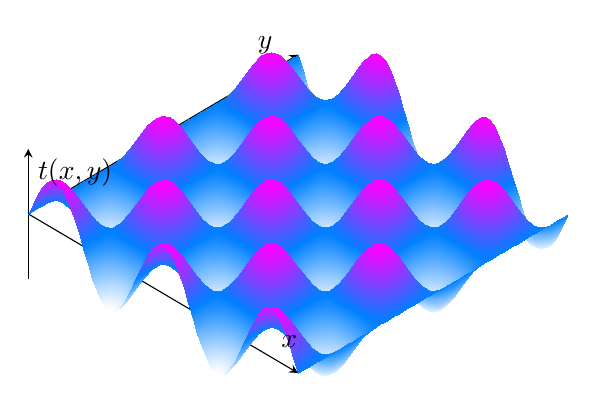
\begin{tikzpicture}
    \begin{axis}[
      view={45}{60},
      colormap/cool,
      xlabel={$x$},
      ylabel={$y$},
      zlabel={$t(x,y)$},
      domain=0:5*pi,
      domain y=0:5*pi,
      samples=60,
      samples y=60,
      mesh/ordering=y varies,
      enlargelimits=true,
      axis lines=middle,
      ticks=none,
      zmin=-0.8, zmax=0.8,
    ]
      \addplot3[
        surf,
        shader=interp,
      ]
      {0.6 * sin(deg(x)) * cos(deg(y))};
    \end{axis}
  \end{tikzpicture}
  \caption{A schematic representation of spacetime as a standing wave. Each spatial coordinate $(x,y)$ exhibits a temporal oscillation, represented on the vertical axis. The oscillatory structure encodes temporal granularity, setting a natural limit to resolution and uncertainty.}
  \label{fig:standing_wave_oscillation}
\end{figure}


\section{Gravity as Temporal Gradients in a Standing Wave Spacetime}

The prevailing view in modern physics treats gravity as a fundamental interaction, possibly mediated by a massless spin-2 boson, the graviton~\cite{Feynman1963,Weinberg1965,wikipediaGraviton}. While mathematically consistent, this picture raises persistent challenges: how could such a mediator act universally on all matter, propagate effects that seem instantaneous across vast distances, and remain both persistent and irreversible if governed by particle exchange? These difficulties motivate a shift in perspective: gravity need not be mediated at all, but may instead emerge from the geometry of time itself.

\subsection{From Mediation to Emergence}

Consider two neighboring regions of spacetime where clocks tick at different rates. A physical object entering such a region will drift toward slower time, not because it is pulled by a force, but because the structure of spacetime itself has a gradient. In this view, gravity is a push into regions of greater temporal dilation, much like fluid flows along a pressure gradient. General Relativity already encodes this behavior mathematically as geodesic motion in curved spacetime~\cite{Einstein1916,MTW1973}; the present model extends that intuition by proposing that curvature is not a passive geometry but an active \emph{temporal gradient}.

\subsection{Temporal Gradients and Free Fall}

Let $\tau(x^\mu)$ represent the proper time measured at spacetime point $x^\mu$. Near mass–energy concentrations, the local rate of time flow decreases, and we may define a temporal gradient as
\[
\nabla_t \equiv \nabla \left( \frac{d\tau}{dt} \right).
\]
This gradient points toward regions where time runs more slowly. Matter responds by accelerating in that direction:
\[
\vec{a} \propto -\nabla_t.
\]
Free fall is therefore not motion under a force, but the natural descent along a temporal slope. The equivalence principle~\cite{Einstein1907,Will2014} follows directly: all matter responds identically to $\nabla_t$, because it is not being acted upon by an external interaction but simply guided by the structure of proper time.

\subsection{Mass, Impedance, and the Higgs Connection}
\label{sec:higgs-impedance}

The Higgs mechanism explains why particles acquire mass through interaction with a pervasive field~\cite{Higgs1964,Englert1964}, yet it offers little intuition for why such a field exists. In the standing wave model of spacetime, a new picture emerges: spacetime itself is a discrete resonant structure, with nodes and antinodes that define fundamental intervals $\Delta x$ and $\Delta t$. Massless particles such as photons traverse this structure without impedance, while massive particles disturb it locally. This disturbance produces resistance to motion---an \emph{impedance}---which manifests as inertia.

In this framework, the Higgs field need not be a separate entity. Rather, it is an emergent feature of the nodal structure of spacetime. Mass is the local impedance of matter against this discrete wave medium, and gravity arises when temporal gradients create regions of least resistance. Matter is effectively pushed toward slower time because that is where motion through the spacetime lattice encounters minimal impedance. Gravity thus becomes a macroscopic consequence of microscopic impedance.

\subsection{Summary: Gravity as an Emergent Push}

In this reframing, gravity is neither a mysterious long-range force nor a quantum exchange. It is the natural flow of matter down temporal gradients in a discrete standing wave spacetime. The Higgs mechanism and gravitational behavior are united under a single structural principle: mass, inertia, and acceleration all originate from the way matter interacts with the temporal fabric of the universe. Gravity, then, is best understood not as attraction, but as an emergent push into slower time.


\section{Black Surfaces and the Critical Warp Limit}

In the standing wave spacetime framework, the extreme warping traditionally attributed to black hole singularities is replaced by a finite, physical surface limit. Rather than diverging to infinite curvature, spacetime exhibits a maximum surface energy density beyond which further stretching is not possible \cite{penrose1965, hawking1970}.

We define the \emph{critical surface energy density} as:
\[
\sigma_{\text{crit}} = \frac{E}{A}
\quad
\text{where}
\quad
E = \text{local energy content},
\quad
A = \text{surface area enclosing the region}.
\]

At $\sigma_{\text{crit}}$, the local standing wave structure reaches its maximum deformation. This implies that a black hole does not harbor a mathematical singularity but terminates at a \emph{Black Surface}---a phase transition boundary beyond which spacetime can no longer sustain additional curvature.

\subsection{Physical Intuition and Mode Filtering}

Spacetime in this picture behaves analogously to an elastic drumhead composed of quantized standing wave nodes. As mass-energy accumulates, the nodes are displaced, producing a local temporal gradient---the origin of gravitational effects. Approaching $\sigma_{\text{crit}}$, the system undergoes a transition similar to a drum tightening: lower-frequency modes can no longer be supported and are expelled, while only higher-frequency oscillations persist.

This expulsion of long-wavelength modes acts as a \emph{high-pass filter} on matter-energy degrees of freedom, resonant with ideas in quasinormal mode analyses \cite{kokkotas1999}. Low kinetic energy matter is squeezed outward, forming a dense shell at the periphery. The Black Surface therefore emerges not as a mathematical artifact but as a physically stable configuration: a shell-like boundary where the discrete standing wave lattice can still sustain oscillation, while the interior flattens into a nearly featureless region.

In this sense, the Black Surface preserves the observable phenomena of horizons and shadows while avoiding infinities. The singularity is replaced by a phase transition in the standing wave structure itself.

\subsection{Observational Anchors}

Remarkably, existing astrophysical measurements hint at this finite limit. Supermassive black holes exhibit average volumetric densities comparable to water \cite{king2006, ozel2010}---orders of magnitude lower than nuclear densities. Such values are consistent with the idea that the interior is not a runaway collapse but instead a regulated region whose warp has saturated at $\sigma_{\text{crit}}$, pushing additional matter outward into the surrounding shell.

\begin{figure}[H]
  \centering
  % --- Row 1 ---
  \begin{subfigure}[b]{0.3\textwidth}
    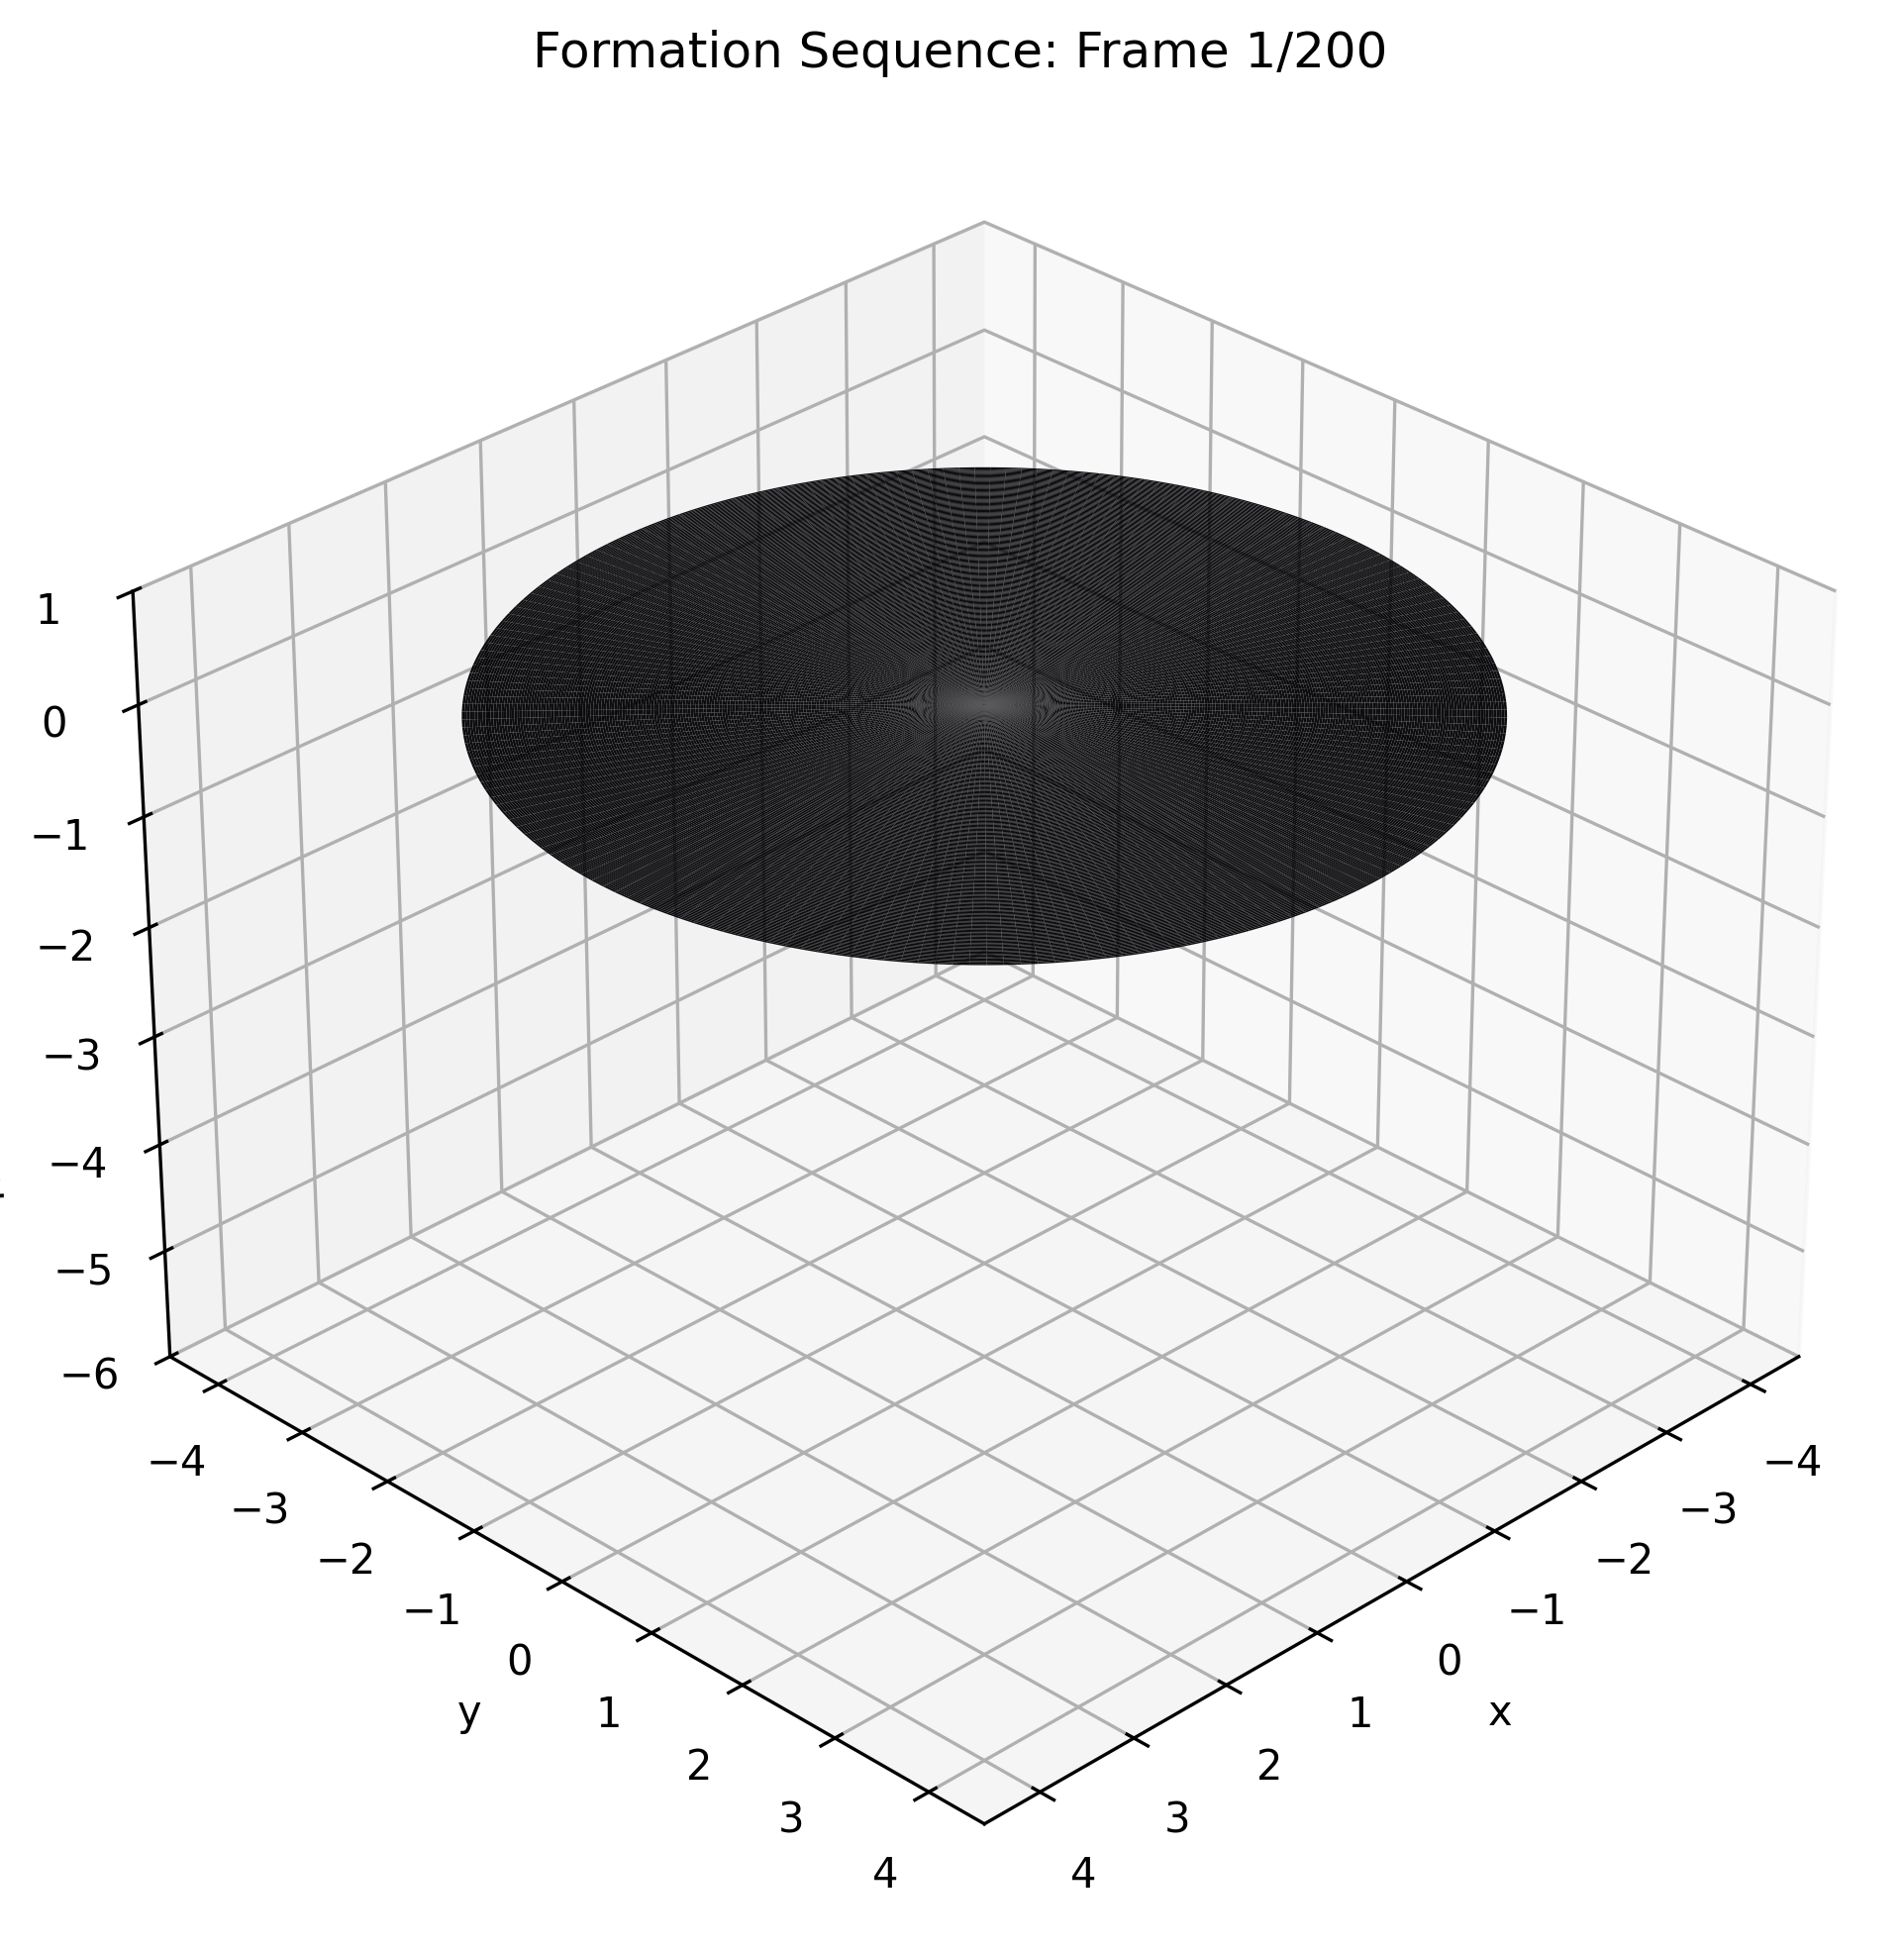
\includegraphics[width=\textwidth]{frame_001.png}
    \caption{Flat spacetime}
  \end{subfigure}
  \hfill
  \begin{subfigure}[b]{0.3\textwidth}
    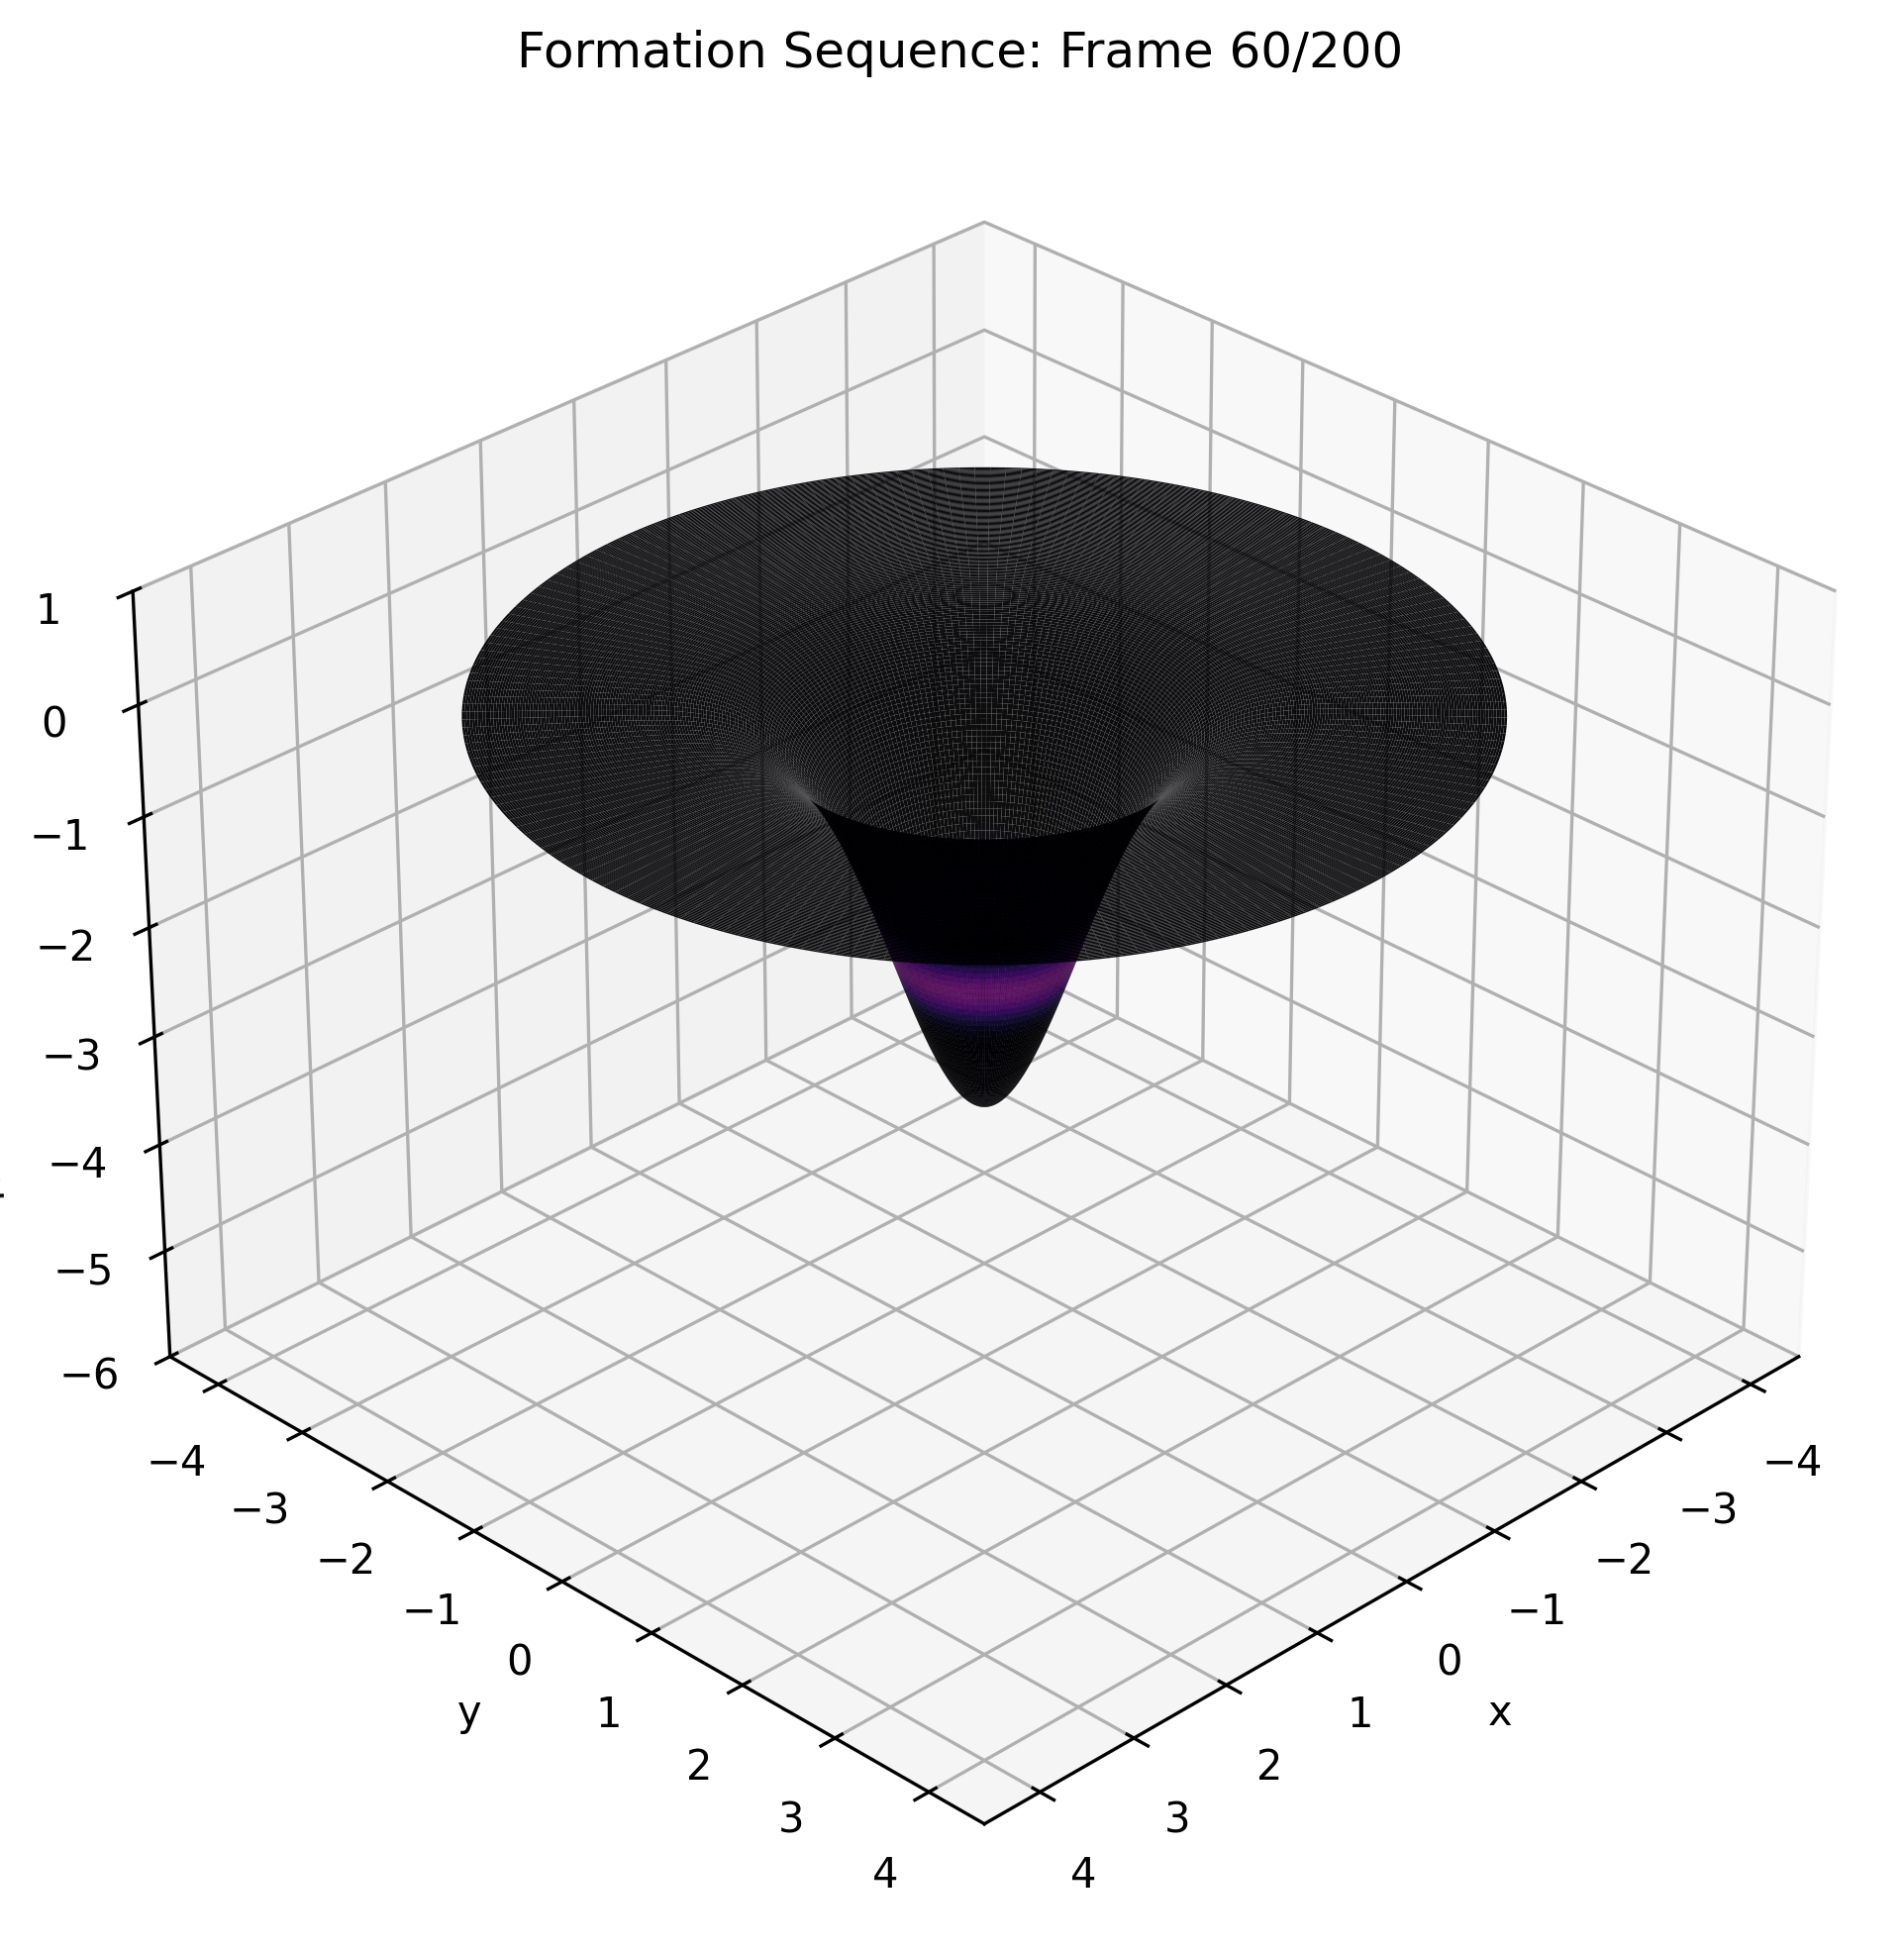
\includegraphics[width=\textwidth]{frame_060.png}
    \caption{Classic warp}
  \end{subfigure}
  \hfill
  \begin{subfigure}[b]{0.3\textwidth}
    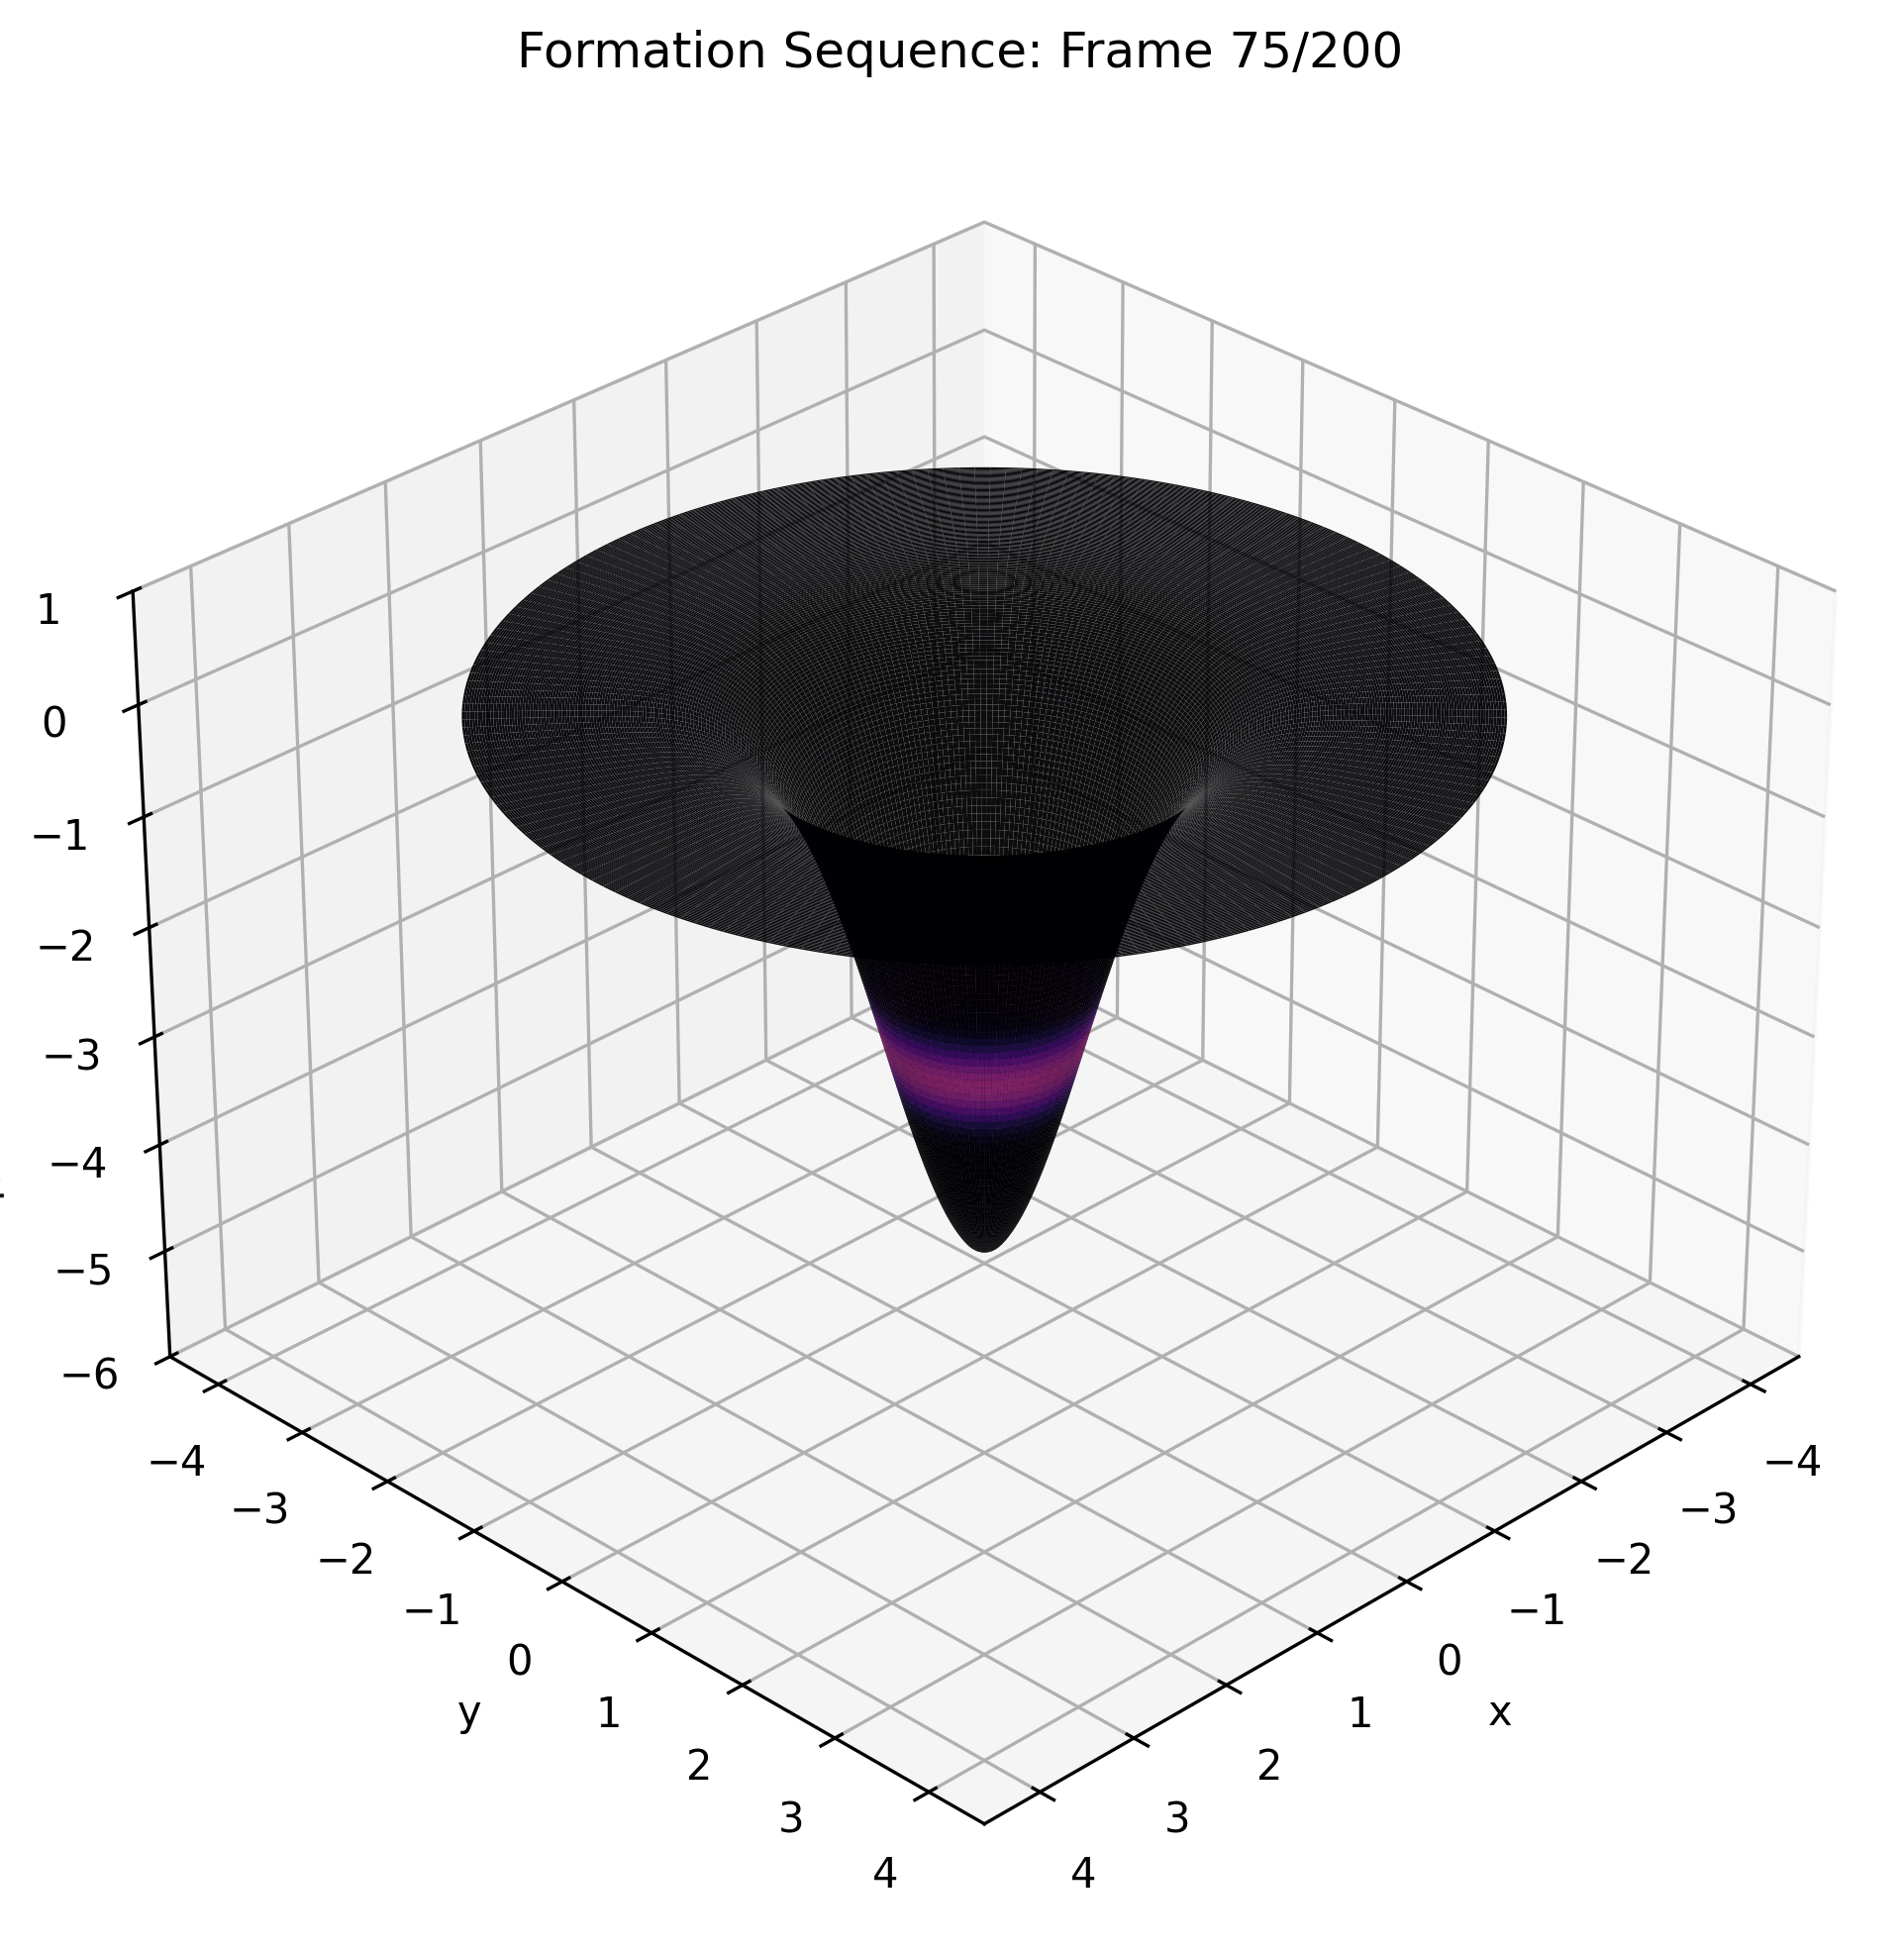
\includegraphics[width=\textwidth]{frame_075.png}
    \caption{Approaching warp limit}
  \end{subfigure}

  \par\vspace{0.5em}

  % --- Row 2 ---
  \begin{subfigure}[b]{0.3\textwidth}
    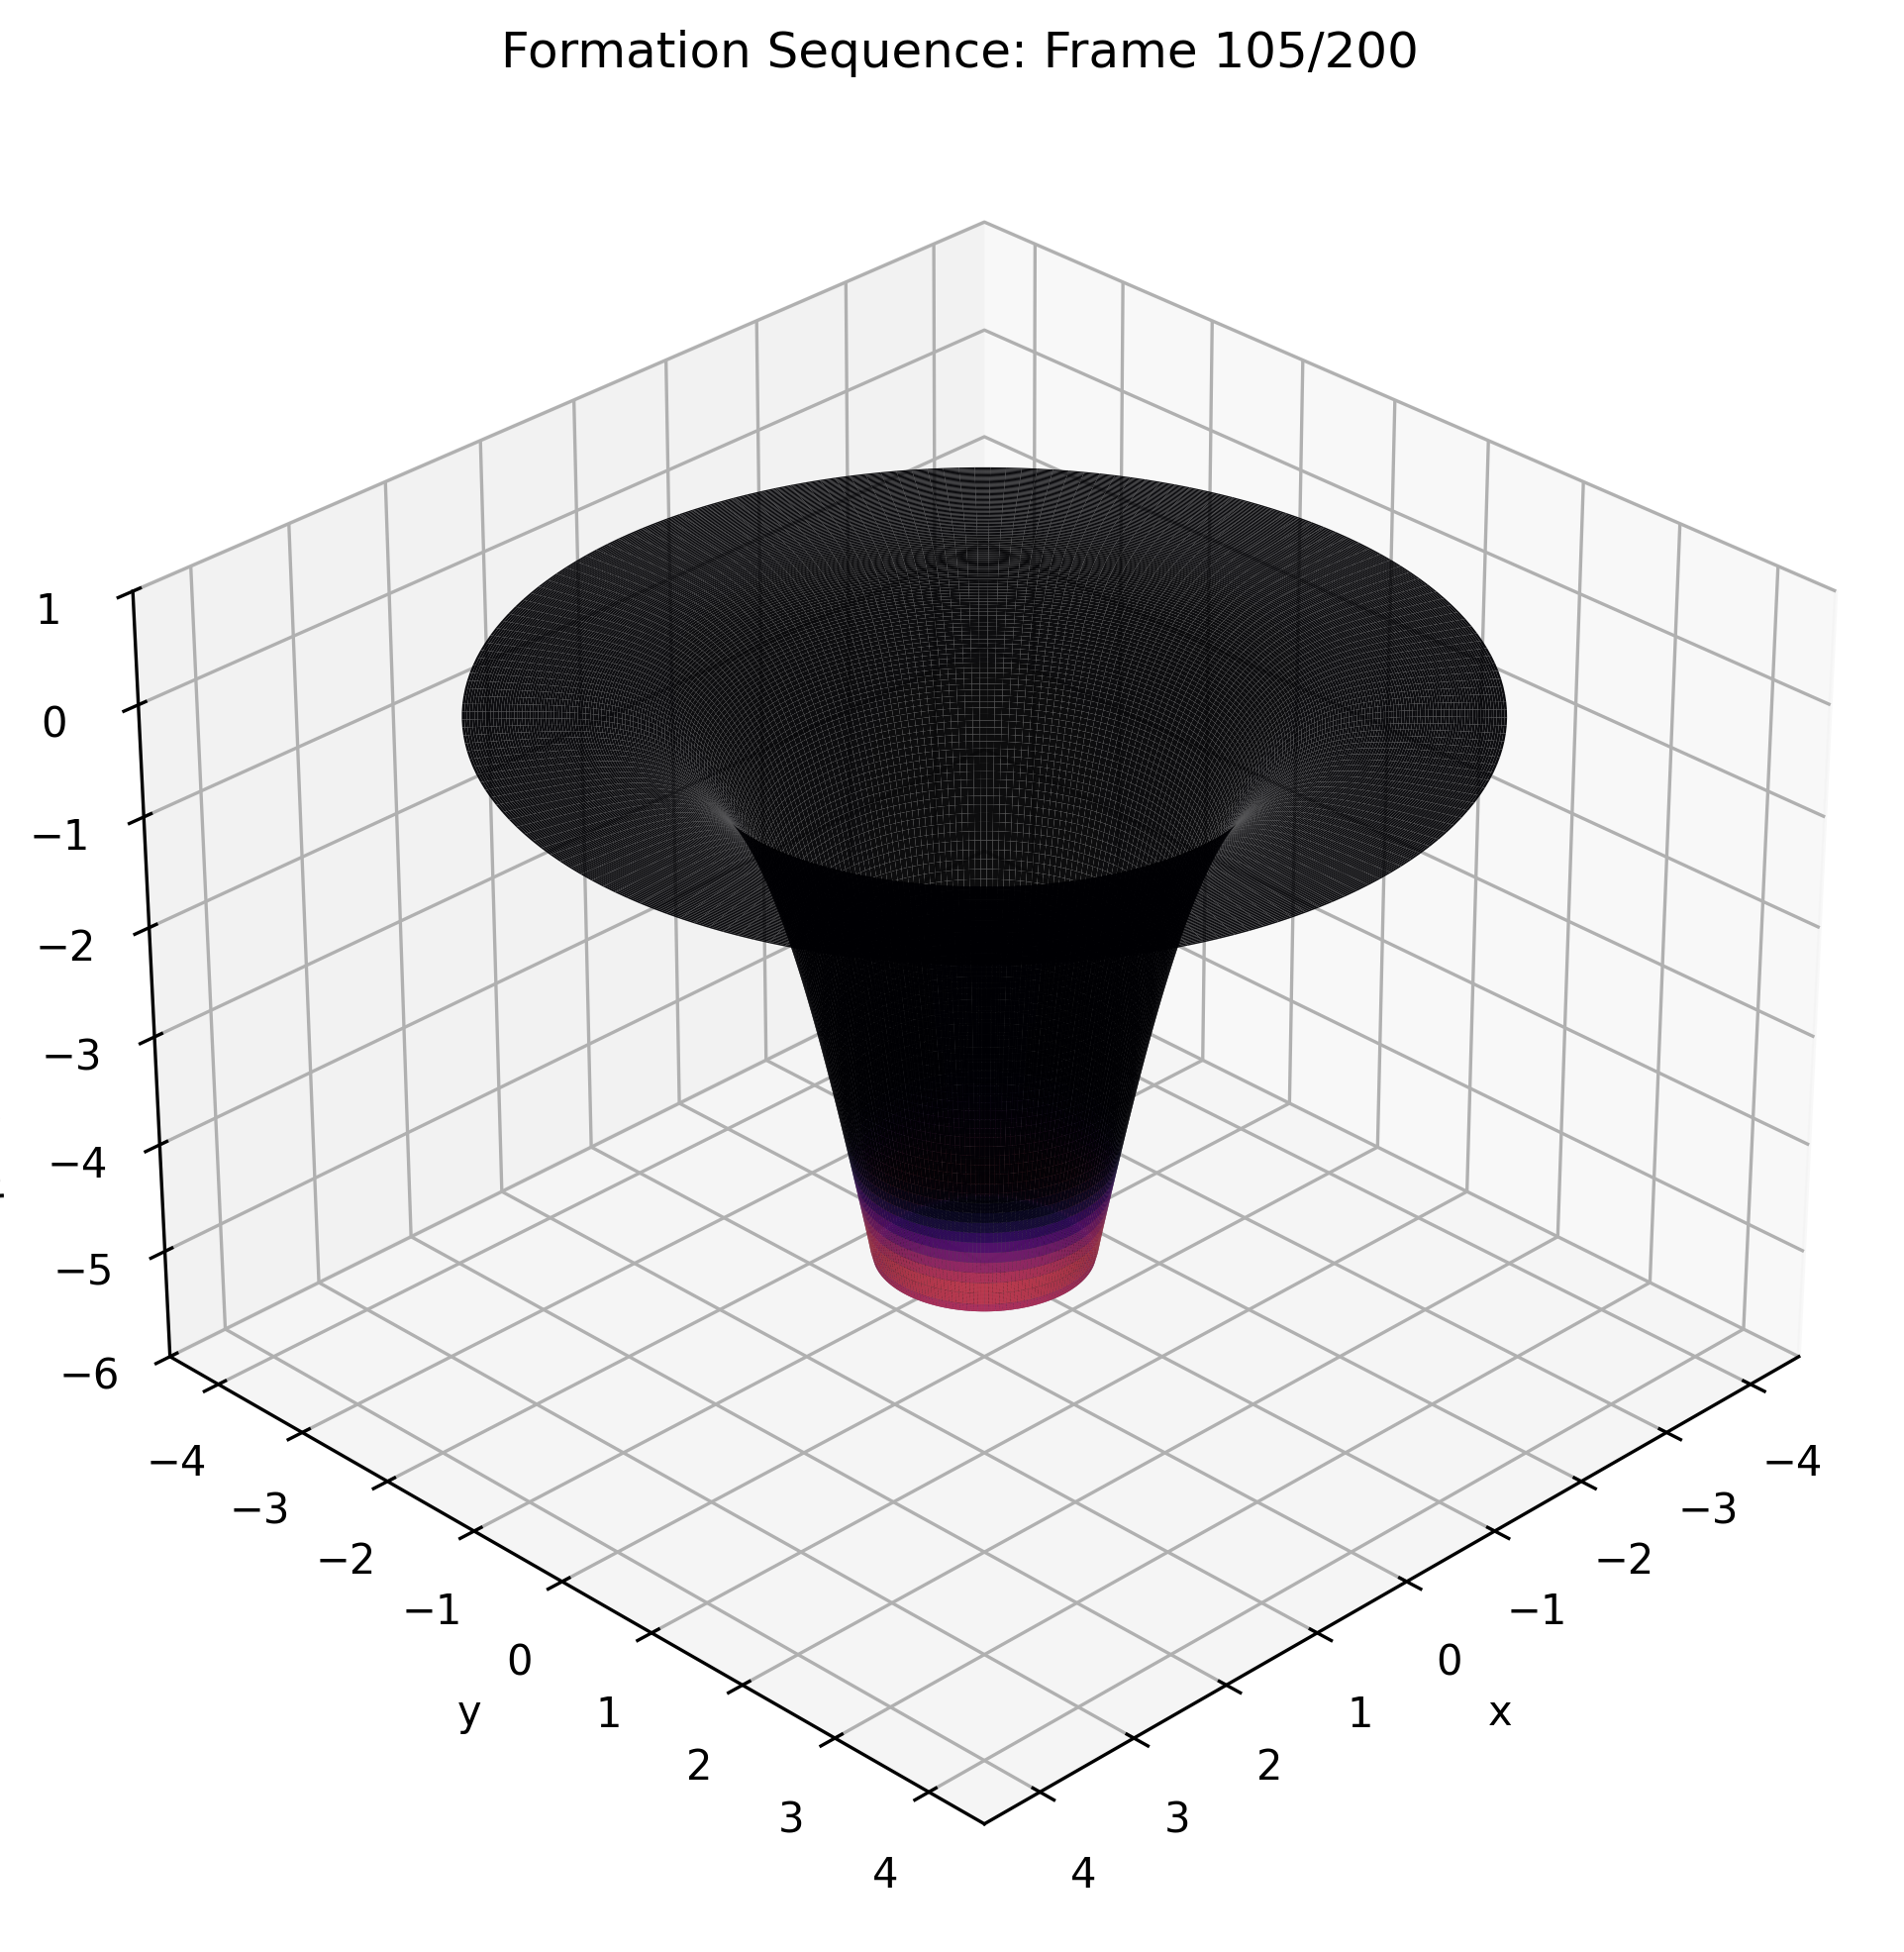
\includegraphics[width=\textwidth]{frame_105.png}
    \caption{Photosphere visible}
  \end{subfigure}
  \hfill
  \begin{subfigure}[b]{0.3\textwidth}
    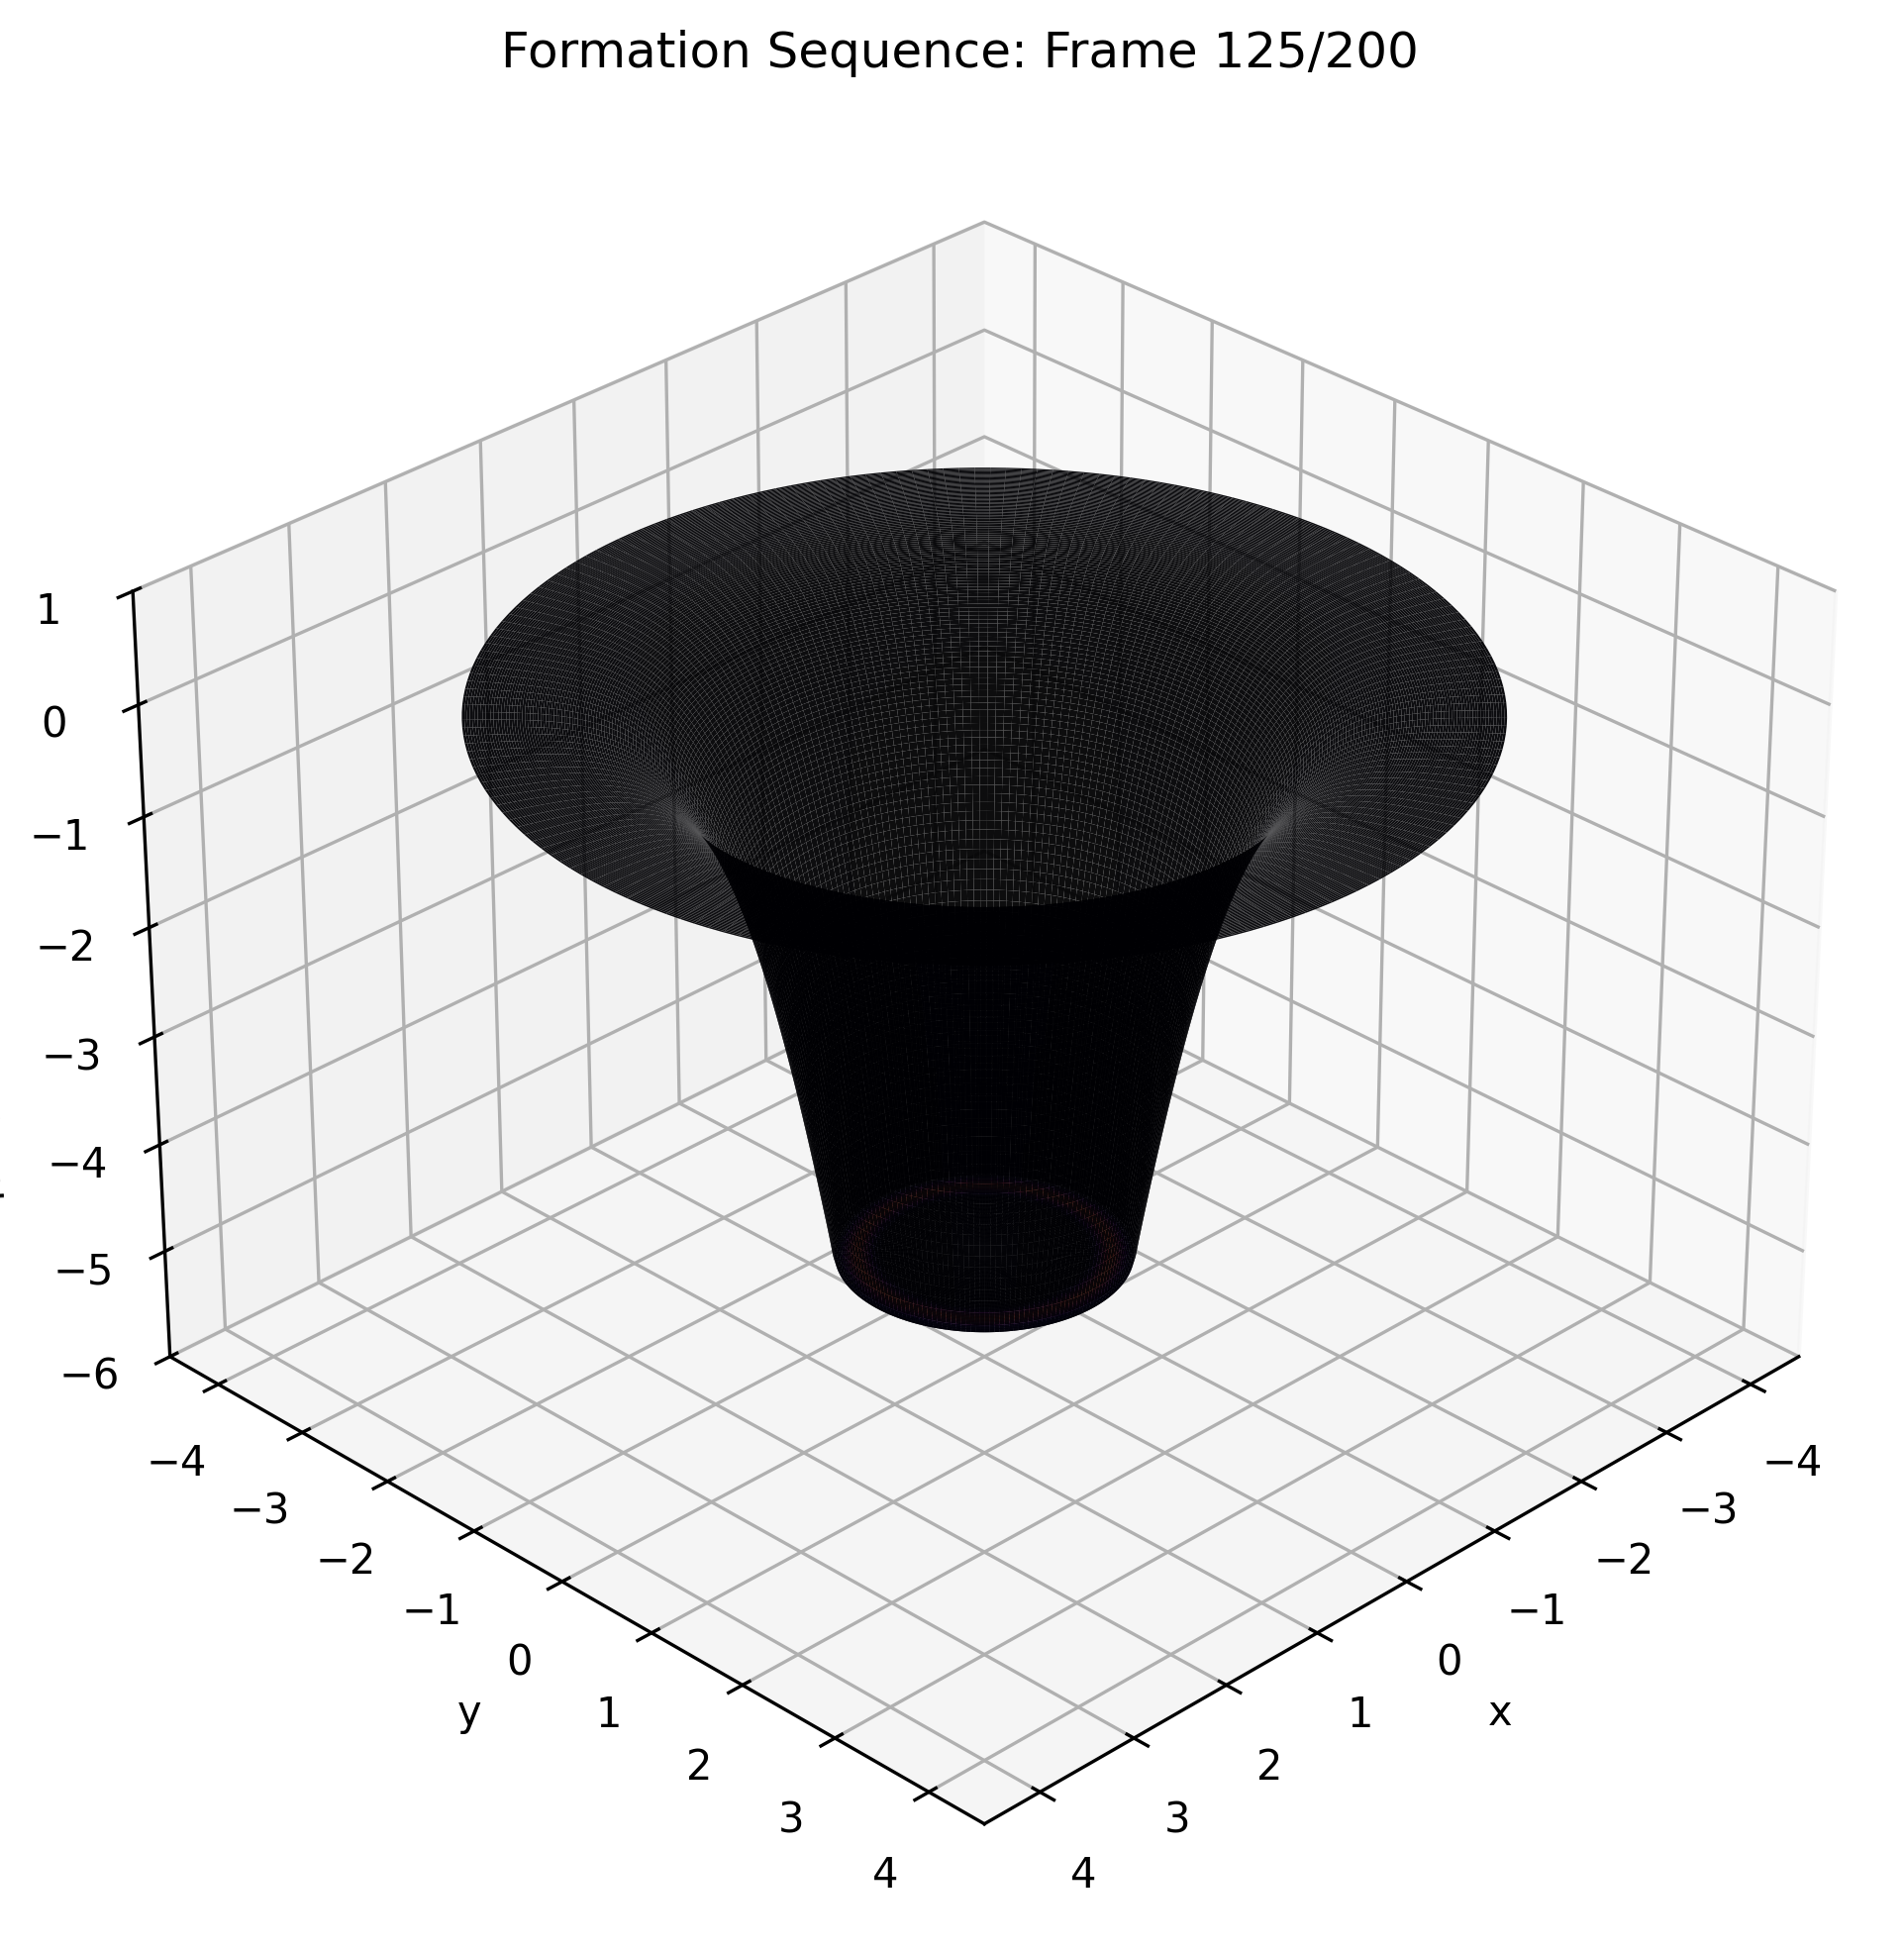
\includegraphics[width=\textwidth]{frame_125.png}
    \caption{Event horizon forms}
  \end{subfigure}
  \hfill
  \begin{subfigure}[b]{0.3\textwidth}
    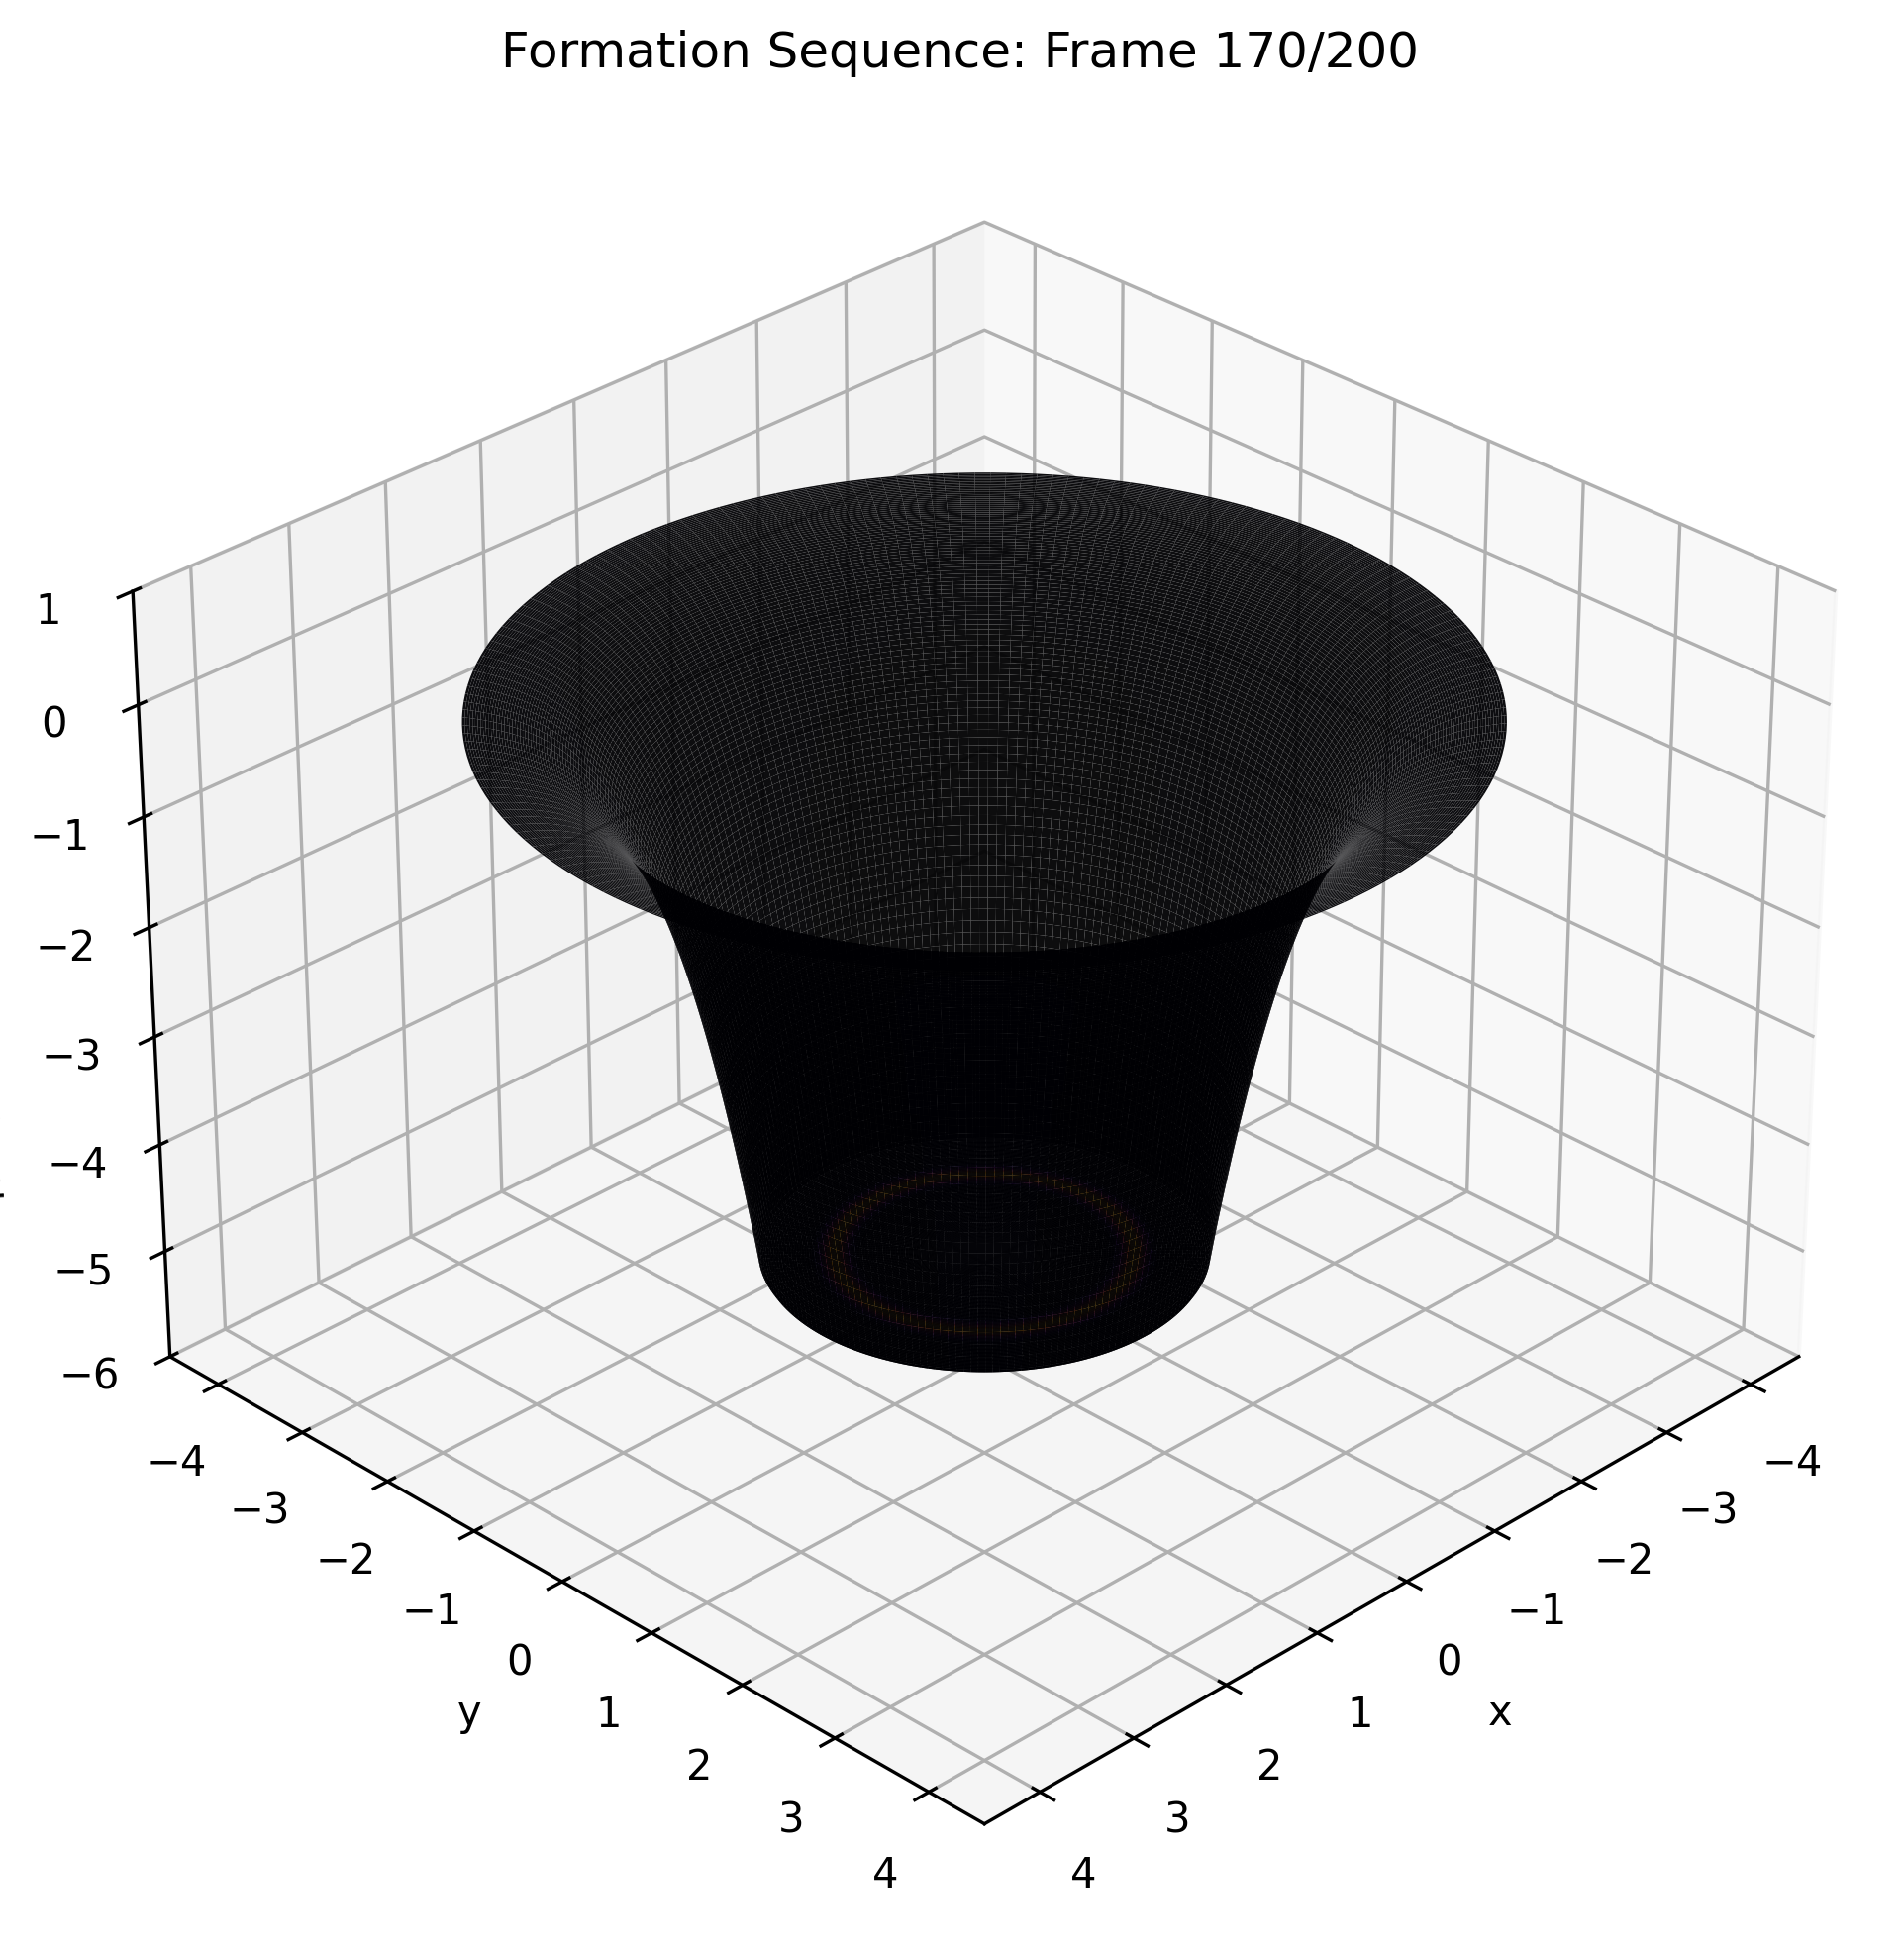
\includegraphics[width=\textwidth]{frame_170.png}
    \caption{Stable shell hidden}
  \end{subfigure}

  \caption{Stages of Black Surface formation in the discrete standing wave model: a smooth progression from flat spacetime through warp limit to stable shell hidden behind the emergent event horizon.}
  \label{fig:black_surface_stages}
\end{figure}

\subsection{Implications for Observables}

By reframing black holes as Black Surfaces, this model preserves the large-scale predictions of general relativity while offering new testable features:
\begin{itemize}
    \item The size and morphology of photon spheres and gravitational shadows \cite{eventhorizon2019}, which may encode the presence of a shell-like surface rather than a pointlike singularity.
    \item Angular momentum constraints (e.g., the Kerr bound) as manifestations of how the standing wave structure resists further stretching.
    \item Potential imprints of surface-mode filtering in gravitational wave spectra or accretion dynamics, where transitions across $\sigma_{\text{crit}}$ could leave observable signatures \cite{abbott2016, cardoso2016}.
\end{itemize}


\cleardoublepage
\part{Mathematical Consequences}

\section{Cosmic Timeline}

\subsection{Looking Backward: Early–Universe Behavior}

In this model, the speed of light is not taken as a fundamental constant but arises from the ratio of spatial to temporal intervals,
\begin{equation}
c \;\equiv\; \frac{\Delta x}{\Delta t}.
\end{equation}
While the fundamental tick of time, $\Delta t$, is assumed invariant, the spatial interval $\Delta x$ scales with the expansion factor $a(t)$. 
As the universe contracts toward the big bang, $\Delta x \to 0$ while $\Delta t$ remains finite, forcing $c$ itself to evolve with cosmic volume. 

Thus, in the limit $a(t) \to 0$, we obtain
\begin{equation}
\lim_{a\to 0} c(V) \;=\; 0,
\end{equation}
so that the \emph{effective} speed of light in the early universe tends toward zero---in stark contrast to the usual intuition of diverging speeds near the big bang.

This inversion has profound consequences:
\begin{itemize}
\item Causal signals in the early universe propagate extremely slowly.  
\item The comoving particle horizon evolves in a radically different manner, directly resolving the horizon problem and removing the need for an \emph{ad hoc} inflationary phase to explain the observed uniformity of the Cosmic Microwave Background.  
\item Interpreting high--redshift events under the constant-$c$ assumption introduces systematic errors that grow exponentially with redshift.  
\end{itemize}

For example, if $c(V) \propto a^{3\alpha}$, then the standard lookback time formula,
\begin{equation}
t_{\rm inferred}(z) = \int_0^z \frac{dz'}{(1+z')\, H(z')},
\end{equation}
must be replaced by
\begin{equation}
t_{\rm true}(z) = \int_0^z \frac{[1+z']^{-3\alpha}}{(1+z')\, H(z')} \, dz' .
\end{equation}
The ratio $t_{\rm true}/t_{\rm inferred}$ falls sharply toward zero as $z$ increases.  
Thus, distant supernovae appear anomalously faint when analyzed under constant-$c$ assumptions, creating the illusion of accelerated expansion even in the absence of dark energy.  
In this view, what standard cosmology interprets as dark energy may be an artifact of treating $c$ as immutable.  

\medskip
To examine these consequences rigorously, we now reformulate the FRW metric and Einstein equations under the condition $c = c(V)$.

\subsection{Modifications to the FRW Metric}

In the standard Friedmann–Robertson–Walker (FRW)~\cite{frw} cosmology, the line element is written as
\begin{equation}
  ds^2 = -c^2 dt^2 + a(t)^2 \left( \frac{dr^2}{1 - k r^2} + r^2 d\Omega^2 \right),
\end{equation}
with constant light speed \(c\). In the standing wave spacetime model, however, the speed of light is not an immutable constant but depends on the volumetric scale of the universe,
\begin{equation}
  c = c(V),
\end{equation}
where \(V\) is the effective spatial volume determined by the scale factor \(a(t)\). Thus the line element becomes
\begin{equation}
  ds^2 = -c(V)^2 dt^2 + a(t)^2 \left( \frac{dr^2}{1 - k r^2} + r^2 d\Omega^2 \right).
\end{equation}

This change has immediate consequences. Proper time and conformal time must be carefully distinguished when \(c\) itself evolves. The conformal time is defined by
%\begin{equation}
%  \eta = \int \frac{c(V)}{a(t)} \, dt,
%\end{equation}
\begin{equation}
\eta = \int \frac{c(V)}{a(t)} \, dt
\label{eq:frw_conformal_time}
\end{equation}
which alters the causal structure of the FRW spacetime. Horizons, particle communication limits, and light cone structures all evolve differently than in the constant-\(c\) case.

\subsection{Einstein Equations with \texorpdfstring{$c(V)$}{c(V)}}

The Einstein field equations,
\begin{equation}
  G_{\mu\nu} \;=\; \frac{8\pi G}{c^4}\,T_{\mu\nu},
\end{equation}
inherit the variability of \(c\).  If \(c = c(V)\), the coupling between geometry and stress–energy becomes time dependent.  This does not break covariance: \(c\) remains a scalar under local Lorentz transformations.  Rather, it introduces an evolving \emph{impedance} in the relationship between curvature and matter, a \textbf{phase–metric coupling} whereby the standing–wave structure of spacetime modulates the strength of interaction between geometry and energy density.

Deriving the modified Friedmann equations, we obtain
\begin{align}
  \left(\frac{\dot{a}}{a}\right)^2 + \frac{k\, c(V)^2}{a^2} &= \frac{8 \pi G}{3}\,\rho, \\
  \frac{\ddot{a}}{a} &= -\frac{4 \pi G}{3}\!\left( \rho + \frac{3p}{c(V)^2} \right).
\end{align}

In the constant-$c$ limit these equations reduce to the standard Friedmann–Robertson–Walker form~\cite{frw}, but with $c(V)$ explicit the balance between density, pressure, and acceleration is altered.  

This modification is not merely formal. Because $c(V)$ also enters the Einstein coupling $\kappa(V) = 8\pi G / c(V)^4$, the effective strength of gravity evolves with cosmic volume. In later sections we will see that this predicts a universe in which gravity was overwhelmingly strong in its earliest epochs, and only appears ``weak'' today because spacetime has expanded.

Previous varying–speed–of–light (VSL) models (e.g.\ \cite{albrecht1999,barrow1999,magueijo2003}) explored whether a time– dependent \(c(t)\) could resolve puzzles such as the horizon and flatness problems.  In those approaches, \(c\) was introduced as an external prescription, a function appended to the equations.

By contrast, in the present framework the variability of \(c(V)\) is inevitable: it follows directly from the geometric structure of spacetime itself.  With \(\Delta t\) invariant and \(\Delta x\) scaling with cosmic volume, the effective propagation speed cannot remain constant.  The result is a dynamical reinterpretation of cosmological evolution in which phenomena usually ascribed to a cosmological constant or inflation may instead reflect the natural evolution of \(c(V)\).

\subsection{Reinterpreting the Cosmological Constant}

When distant Type Ia supernovae were first observed to be dimmer than expected, the conclusion was that the universe’s expansion was accelerating \citep{perlmutter1999, riess1998}. This led directly to the resurrection of Einstein’s cosmological constant \( \Lambda \), rebranded as Dark Energy, comprising nearly 70\% of the cosmic energy budget \citep{planck2018}.

But in the discrete standing wave spacetime model, this interpretation may not be required. If the speed of light grows with the volume of the universe, i.e.
\begin{equation}
  c = c(V), \qquad \frac{dc}{dV} > 0, \qquad \frac{d^2c}{dV^2} < 0,
\end{equation}
then signals from distant supernovae will appear redshifted and dimmer not because of acceleration, but because our interpretation assumes constant light speed. The observed dimming may instead be a signature of a \textbf{time-varying propagation speed in a stretching medium}. Correcting the luminosity–distance relation to account for \(c(V)\) may eliminate or greatly reduce the apparent acceleration. The ``Dark Energy'' problem becomes a bookkeeping error of interpretation.

\begin{quote}
\textit{Einstein’s greatest mistake may have been doubting his deepest intuition.}
\end{quote}

This reinterpretation also directly addresses the infamous \textit{Vacuum Energy Catastrophe}. In standard treatments, quantum field theory predicts vacuum energy densities \(10^{120}\) times larger than observed. But if the cosmological constant is not a true energy density, but an artifact of misinterpreting signals under constant \(c\), then the contradiction vanishes \citep{weinberg1989}.

\subsection{Reassessing the Horizon Problem}

In standard cosmology, the so-called \emph{horizon problem} arises because the Cosmic Microwave Background (CMB) is observed to be remarkably uniform in temperature across regions that, under the constant-$c$ assumption, appear causally disconnected at recombination \cite{smoot1992}. The conventional reasoning is that there was insufficient time for thermalization to occur, motivating an inflationary phase to explain this uniformity \cite{liddle2000}.

This argument relies on three key assumptions:
\begin{itemize}
\item The speed of light \(c\) is constant throughout cosmic history.
\item All energy resides in matter or radiation; spacetime itself is passive.
\item Thermal equilibrium requires direct causal contact between regions.
\end{itemize}

While these considerations make the uniformity of the CMB puzzling under standard assumptions, the standing-wave spacetime model offers a different perspective.

In this framework, spacetime carries energy, which is transferred uniformly into matter as the universe expands, according to the evolving mass-energy relation
\begin{equation}
E(V) = m\,c(V)^2.
\end{equation}
Because this energy distribution is homogeneous, matter inherits thermal uniformity naturally, independent of causal contact or the size of the particle horizon.

\begin{figure}[h!]
\centering
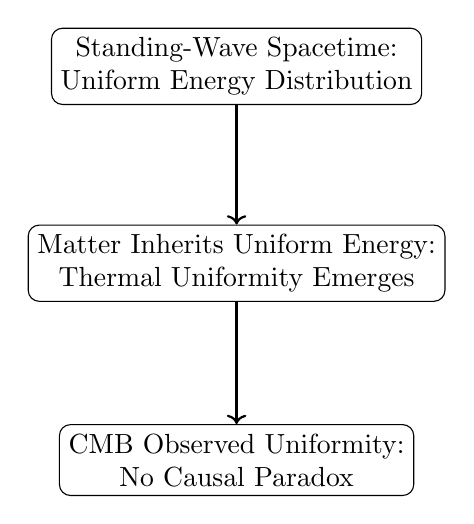
\begin{tikzpicture}[node distance=2.5cm, every node/.style={draw, rounded corners, align=center}]
\node (spacetime) {Standing-Wave Spacetime:\\Uniform Energy Distribution};
\node (matter) [below of=spacetime] {Matter Inherits Uniform Energy:\\Thermal Uniformity Emerges};
\node (cmb) [below of=matter] {CMB Observed Uniformity:\\No Causal Paradox};
\draw[->, thick] (spacetime) -- (matter);
\draw[->, thick] (matter) -- (cmb);
\end{tikzpicture}
\caption{Horizon problem “resolved”: thermal uniformity of matter and the CMB emerges naturally from uniform energy distribution in standing-wave spacetime.}
\label{fig:horizon_flow}
\end{figure}

Minor quantum fluctuations in matter are superimposed on this uniform background, providing seeds for the anisotropies that later grow into galaxies and clusters \cite{mukhanov1992}. These fluctuations coexist with an overall thermal uniformity and do not contradict the mechanism: the uniform energy transfer sets the baseline, while quantum perturbations generate structure.

Thus, under this framework, the horizon problem is no longer a puzzle. Uniformity of the CMB is a direct consequence of the underlying geometry and energy distribution of spacetime. What standard cosmology treats as a “problem” becomes instead a prediction: thermal homogeneity is expected across the observable universe without requiring inflation or artificially adjusting the propagation speed of light.

\subsection{Baryon Acoustic Oscillations and the Poisson Imprint}

Baryon Acoustic Oscillations (BAO) provide a snapshot of the primordial density field at the epoch of recombination. In standard cosmology, the sound horizon at that time, $r_s$, sets the scale of the oscillations, which then seed the later formation of galaxies and clusters \cite{eisenstein2005,white2005}.  

\begin{figure}[h!]
\centering
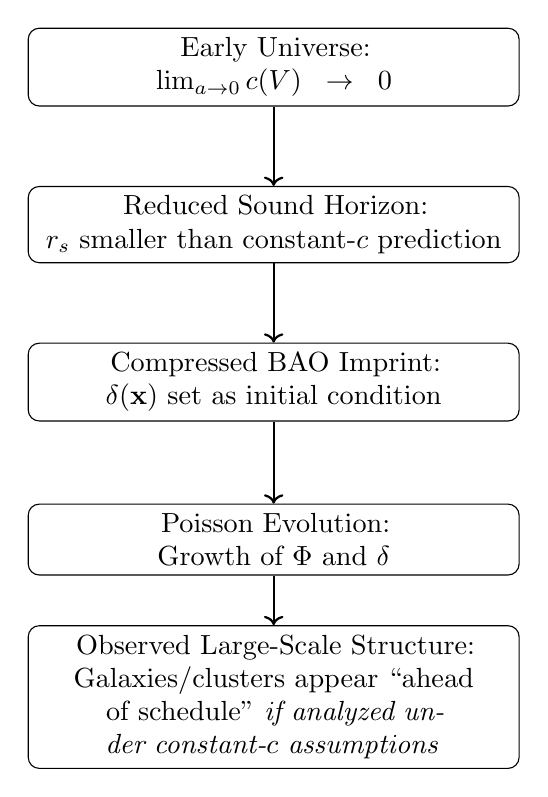
\begin{tikzpicture}[node distance=2cm, every node/.style={draw, rounded corners, align=center, text width=6cm}]
% Nodes
\node (c0) {Early Universe:\\$\lim_{a\to 0} c(V) \to 0$};
\node (sound) [below of=c0] {Reduced Sound Horizon:\\$r_s$ smaller than constant-$c$ prediction};
\node (bao) [below of=sound] {Compressed BAO Imprint:\\$\delta(\mathbf{x})$ set as initial condition};
\node (poisson) [below of=bao] {Poisson Evolution:\\Growth of $\Phi$ and $\delta$};
\node (structure) [below of=poisson] {Observed Large-Scale Structure:\\Galaxies/clusters appear ``ahead of schedule'' \emph{if analyzed under constant-$c$ assumptions}};
% Arrows
\draw[->, thick] (c0) -- (sound);
\draw[->, thick] (sound) -- (bao);
\draw[->, thick] (bao) -- (poisson);
\draw[->, thick] (poisson) -- (structure);
\end{tikzpicture}
\caption{Causal chain connecting early-universe behavior of $c(V)$ to observed large-scale structure. 
A smaller early sound horizon compresses the BAO scale, seeding density perturbations. 
When interpreted under constant-$c$ cosmology, the resulting structures appear ``too early,'' though they arise naturally in the variable-$c$ framework.}
\label{fig:BAO_flow}
\end{figure}

In the standing wave spacetime model, the effective speed of light in the early universe is reduced since it is determined by the underlying spatial geometry,
\begin{equation}
c(V) \to 0 \quad \text{as} \quad a(t) \to 0,
\end{equation}
resulting in a correspondingly smaller sound horizon. The BAO imprint in the density field is therefore compressed relative to what would be inferred under a constant-$c$ assumption.

The Poisson equation,
\begin{equation}
\nabla^2 \Phi = 4 \pi G a^2 \rho \, \delta,
\end{equation}
evolves the initial density perturbations into the large-scale structure observed today \cite{peebles1980}. Because $\delta(\mathbf{x})$ carries the compressed BAO signature, structure formation proceeds on a timeline that appears accelerated if interpreted with constant $c$. 

Observationally, this provides a natural explanation for why galaxies and clusters in the early universe seem ``ahead of schedule'' \cite{adams2023, naidu2022}---they are not forming unusually fast; rather, the effective early-universe clock runs slower in this model.

Thus, what appears observationally as a tension with $\Lambda$CDM and a driver for dark matter or dark energy can instead be reframed as a natural outcome of a variable-$c(V)$ early universe.

\subsection{Summary}

The FRW metric, once modified to include a variable speed of light, provides a natural mechanism for reproducing the apparent acceleration of the universe without requiring Dark Energy. The reinterpretation is consistent with covariance, alters the Einstein equations in a physically transparent way, and suggests fresh perspectives on BAO, CMB horizons, and the Poisson-governed growth of density perturbations. This framework thus offers a mathematically tractable and observationally testable alternative to the cosmological constant paradigm.


\section{Energy as the Universal Currency}

\subsection{Lorentz Invariance and the Emergence of \texorpdfstring{$c$}{c}}

A natural objection to any theory with a variable speed of light is the possible violation of Lorentz invariance. The standing-wave spacetime model, however, preserves \emph{local} Lorentz symmetry while providing a physical basis for the emergence of $c$.

The model introduces a natural node structure defined by characteristic intervals of space $\Delta x$ and time $\Delta t$. Their ratio directly yields the local speed of light,
\begin{equation}
c = \frac{\Delta x}{\Delta t}.
\end{equation}
As the universe expands, $\Delta t$ remains fixed as a fundamental measure of change, while $\Delta x$ grows with the volume of space. This leads to a slow global evolution of $c$, but one that leaves local physics unaffected.

Locally, in a tangent Minkowski frame, the metric retains the standard form,
\begin{equation}
ds^2 = -c_{\text{local}}^2 d\tau^2 + dx^2 + dy^2 + dz^2,
\end{equation}
with $c_{\text{local}}$ invariant for all observers. All experimentally tested relativistic phenomena---time dilation, length contraction, mass–energy equivalence---remain intact. The variation arises only in comparing widely separated epochs of cosmic history:
\begin{equation}
  c = c(V), \qquad \frac{dc}{dV} > 0, \qquad \frac{d^2c}{dV^2} < 0,
\end{equation}

In this sense, Lorentz invariance is not broken but reinterpreted. The constancy of $\Delta t$ and the evolution of $\Delta x$ follow necessarily from the standing-wave structure of spacetime, grounding $c$ in the geometry of the universe itself rather than treating it as a fundamental axiom.

\subsection{Einstein Equations with a Variable Coupling}

In general relativity, the Einstein field equations~\cite{misner1973}  
\begin{equation}
  G_{\mu\nu} = \frac{8\pi G}{c^4} T_{\mu\nu},
\end{equation}
show that the speed of light does more than set units: it enters as part of the coupling constant that links matter to geometry~\cite{albrecht1999}. The standing-wave spacetime model modifies this structure by allowing
\begin{equation}
  c = c(V),
\end{equation}
so that the effective coupling evolves with the cosmic volume.

This has two key consequences:

\begin{enumerate}
  \item \textbf{Time-dependent impedance of spacetime.} Spacetime geometry does not respond to stress–energy with fixed strength. Instead, the ratio of curvature to energy density changes as the universe expands, reflecting a dynamical impedance of spacetime itself.
  \item \textbf{Redefinition of energy density.} Stress–energy conservation,
  \begin{equation}
    \nabla^\mu T_{\mu\nu} = 0,
  \end{equation}
  still holds by construction. But the energy associated with matter now includes a factor of $c(V)^2$, so that the very definition of energy density evolves with cosmic volume, consistent with
  \begin{equation}
    E(V) = m\,c(V)^2.
  \end{equation}
\end{enumerate}

It is useful to write the volume-dependent coupling explicitly as
\begin{equation}
  \kappa(V) = \frac{8 \pi G}{c(V)^4},
\end{equation}
so that
\begin{equation}
  G_{\mu\nu} = \kappa(V) T_{\mu\nu}.
\end{equation}
As $c(V)$ grows with the expansion, $\kappa(V)$ decreases, making the effective strength of gravity diminish over cosmic time. This provides a natural dynamical explanation for the relative weakness of gravity compared to the other forces, without requiring fine-tuning of constants.

\bigskip

This reframing carries a profound implication: the apparent weakness of gravity is not a timeless fact of nature but a dynamical property of the universe’s volume. As $c(V)$ grows with expansion, the effective coupling $\kappa(V)$ falls, so spacetime today is far less responsive to stress–energy than it was in the early cosmos. Conversely, as $c(V)\to 0$ near the origin, $\kappa(V)\to\infty$, and gravity becomes overwhelmingly strong. 

What we call the ``weakest force’’ is therefore a moving target, tied to cosmic chronology rather than to immutable constants. Gravity is not born weak; it fades with time. This perspective challenges the conventional hierarchy problem and suggests that the relative feebleness of gravity compared to the other interactions is simply a measure of how large and old the universe has become.

\subsection{Alternative Derivation via the Action Principle}

The same conclusion can be obtained from the Einstein–Hilbert action~\cite{waldGR1984,Carroll2004}:
\begin{equation}
  S = \frac{c^3}{16 \pi G} \int R \sqrt{-g} \, d^4x + S_{\text{matter}}.
\end{equation}
If \(c = c(V)\), both the prefactor \(c^3\) and the scaling of the matter sector acquire explicit volume dependence. Variation of this action yields Einstein equations with an evolving coupling \(\kappa(V)\), consistent with the analysis above~\cite{albrecht1999}.

Unlike the standard case, additional boundary contributions appear when varying a time-dependent \(c\). These terms may be linked to horizon evolution and vacuum structure, suggesting a deeper connection between cosmic expansion, particle creation, and the effective energy content of spacetime.

\subsection{Rest Energy and the Energy--Volume Relation}

The volume dependence of the speed of light modifies the equivalence between mass and energy. For a particle of invariant rest mass \(m\), the rest energy becomes
\begin{equation}
  E(V) = m \, c^2(V).
\end{equation}
Mass itself is not changing; rather, the energy equivalence scale evolves with cosmic volume. This shift may be interpreted as a form of \emph{temporal pressure}: the gradient in the rate of time progression across spacetime acts as an effective pressure, driving matter toward regions of slower time (the phenomenon we perceive as gravity) while simultaneously rescaling its energy equivalence.

If rest energy grows with \(c(V)\), energy conservation requires that this increase draw from a physical reservoir. We posit that the standing-wave fabric of spacetime itself stores energy, from which matter continuously extracts rest-energy. In the continuity equation,
\begin{equation}
\frac{d\rho_{\rm m}}{dt} + 3 H \rho_{\rm m} = Q(a) \, ,
\end{equation}
a source term \(Q(a)\) naturally arises, with
\begin{equation}
Q(a) \sim \frac{d}{dt}\big[n_m m c^2(a)\big],
\end{equation}
where \(n_m\) is the comoving number density. This mechanism uniformly deposits energy throughout space, consistent with the observed isotropy of the cosmic microwave background.

For a power-law ansatz $c(a) = c_0 a^{3\alpha}$, the matter density evolves as
\begin{equation}
\rho_{\rm m}(a) \propto a^{-3} c^2(a) = a^{-3 + 6\alpha},
\end{equation}
recovering the same scaling, but now endowed with a direct energetic interpretation.

Finally, the functional form of \(c(V)\) must satisfy
\begin{equation}
  c = c(V), \qquad \frac{dc}{dV} > 0, \qquad \frac{d^2c}{dV^2} < 0,
\end{equation}
ensuring that \(c\) always increases with cosmic volume, but at a decelerating rate. Today the change is imperceptible locally, though its signature remains in the light from distant epochs, where the slower early-\(c\) regime played a dominant role in the universe’s energetic evolution.

\subsection{Recasting the Friedmann Energy Budget}

The Friedmann equation in standard cosmology reads
\begin{equation}
\left(\frac{\dot{a}}{a}\right)^{2} = \frac{8 \pi G}{3} \left( \rho_{m} + \rho_{\gamma} + \rho_{\Lambda} \right) - \frac{k}{a^{2}} .
\end{equation}
with densities scaling as
\begin{align}
\rho_{m}(a) &\propto a^{-3}, &
\rho_{\gamma}(a) &\propto a^{-4}, &
\rho_{\Lambda} &\approx \text{const}.
\end{align}

If instead $c = c(V)$, these relations no longer hold. Matter density acquires a time-dependent factor,
\begin{equation}
\rho_{m}(a, V) = \frac{m c^{2}(V)}{a^{3}} ,
\end{equation}
while radiation scales as
\begin{equation}
\rho_{\gamma}(a, V) \sim \frac{c(V)}{a^{4}} .
\end{equation}
Even the vacuum term may be interpreted as an impedance property of spacetime,
\begin{equation}
\rho_{\Lambda}(V) \sim f\!\left(c(V)\right),
\end{equation}
with form set by the phase–metric coupling of the standing wave background. The traditional separation into radiation-, matter-, and dark-energy–dominated eras is thus replaced by a coupled evolution controlled by $c(V)$.

\subsection{Implications for Equality Epochs}

Matter–radiation equality is normally set by
\begin{equation}
\rho_{m}(a) = \rho_{\gamma}(a) .
\end{equation}
With $c(V)$ this becomes
\begin{equation}
\frac{m c^{2}(V)}{a^{3}} = \frac{c(V)}{a^{4}} ,
\end{equation}
leading to
\begin{equation}
a_{\text{eq}} \sim \frac{1}{m c(V)} .
\end{equation}
The epoch of equality is no longer fixed by microphysical constants but drifts with the cosmic evolution of $c(V)$. A rapidly increasing $c(V)$ pushes equality to smaller $a$, delaying matter domination and the onset of large-scale structure. A more gradual evolution accelerates it. The observed ``early galaxy problem'' thus becomes diagnostic of the slope of $c(V)$ rather than an anomaly.

\subsection{Summary and Connections to Spacetime Impedance}

In this section we have seen how the evolution of $c(V)$ provides a unified description of energy flow, rest-mass scaling, and the apparent anomalies in cosmic expansion. Matter gains energy from the underlying standing-wave structure of spacetime, producing the observed uniformity and shaping the growth of structure. 

The qualitative mechanism linking mass, inertia, and temporal gradients was discussed in Part~II (Section~\ref{sec:higgs-impedance}), where we introduced the notion of spacetime impedance as the origin of the Higgs effect. Here, that framework is extended quantitatively: $c(V)$ sets the energy scale, $\kappa(V)$ modulates gravitational coupling, and $Q(a)$ formalizes the extraction of energy from spacetime.

Together, these ideas provide a consistent energetic picture that naturally transitions to the discussion of Black Surfaces and the resolution of GR, QM, and information tensions.


\section{High-Energy Consequences: Black Surfaces}

The evolution of rest energy in a standing-wave spacetime destabilizes the classical notion of collapse. In conventional general relativity, increasing density drives curvature to infinity at a singularity. In our framework, increasing \(c(V)\) drives the system toward a critical surface energy density,
\begin{equation}
\sigma_{\rm crit} = \frac{E}{A} \sim \frac{m c^2(V)}{A}.
\end{equation}
Once reached, further compression triggers a phase transition: the formation of a \emph{Black Surface}. This replaces the singularity with a stable impedance boundary, tying the endpoint of collapse directly to the structure of spacetime and its standing-wave properties.

\subsection{Static Thin-Shell Model and Israel Junction Conditions}

To provide a mathematical foundation, consider a static, spherically symmetric thin shell in vacuum. The spacetime is split into interior and exterior regions:
\begin{itemize}
    \item \textbf{Interior:} Flat Minkowski space,
    \[ 
    ds^2_{\rm in} = -dt^2 + dr^2 + r^2 d\Omega^2.
    \]
    \item \textbf{Exterior:} Schwarzschild spacetime,
    \[
    ds^2_{\rm out} = -\left(1 - \frac{2GM}{r}\right) dt^2 + \left(1 - \frac{2GM}{r}\right)^{-1} dr^2 + r^2 d\Omega^2.
    \]
\end{itemize}

Matching at the shell radius \(r=R\) requires continuity of the induced metric, while the jump in extrinsic curvature gives the surface stress-energy tensor \(S_{ab}\) via the Israel junction conditions:
\[
[K_{ab}] - h_{ab}[K] = -8\pi G S_{ab}.
\]

For a static shell:
\begin{align*}
\sigma &= -\frac{1}{4\pi R} \left( \sqrt{1 - \frac{2GM}{R}} - 1 \right),\\
P &= \frac{1}{8\pi R} \left( \frac{1 - GM/R}{\sqrt{1 - 2GM/R}} - 1 \right),
\end{align*}
where \(\sigma\) is surface energy density and \(P\) the transverse pressure. As \(R \to 2GM\),  the shell mimics the Schwarzschild horizon, with \(\sigma\) and \(P\) diverging, reproducing the classical horizon location, but the interior remains flat---no singularity forms.

\subsection{Rotating Black Surfaces: Oblate Shells and Kerr Metric}

For rotation, the exterior Schwarzschild metric is replaced with the Kerr metric in Boyer--Lindquist coordinates:
\begin{align*}
ds^2 &= -\left(1 - \frac{2Mr}{\Sigma}\right) dt^2 - \frac{4Mar\sin^2\theta}{\Sigma} dt\, d\phi + \frac{\Sigma}{\Delta} dr^2 + \Sigma d\theta^2 \\
&\quad + \left(r^2 + a^2 + \frac{2Ma^2 r \sin^2\theta}{\Sigma} \right) \sin^2\theta\, d\phi^2,\\
\Sigma &= r^2 + a^2 \cos^2\theta, \quad \Delta = r^2 - 2Mr + a^2, \quad a = \frac{J}{M}.
\end{align*}

Oblate spheroidal coordinates are chosen to ensure that the interior matches the Kerr exterior on the shell while maintaining flatness at the center.  The oblate shell's interior is expressed as follows:
\[
ds^2 = -dt^2 + \frac{a^2(\xi^2 + \eta^2)}{\xi^2 + 1} d\xi^2 + \frac{a^2(\xi^2 + \eta^2)}{1 - \eta^2} d\eta^2 + a^2 (\xi^2 + 1)(1 - \eta^2) d\phi^2,
\]
with shell at \(\xi = \xi_0\). Transformations map \((\xi,\eta)\) to standard spherical coordinates as \(a \to 0\), confirming smooth recovery of spherical Minkowski spacetime.

The cross-term responsible for frame dragging in the Kerr metric is
\begin{equation}
g_{t\phi} = - \frac{2 M a r \sin^2\theta}{\Sigma}
\end{equation}
where $M$ is the mass, $a = J/M$ is the Kerr spin parameter, and $\theta$ is the polar angle. This term encodes the “twist” of spacetime due to rotation.

Frame dragging naturally emerges from the rotational junction: the \(g_{t\phi}\) term encodes the “twist” of inertial frames induced by the shell's angular momentum. This arises purely from geometric continuity and rotational symmetry, with no exotic matter or singularity needed.

\subsection{Effective Speed of Light Inside Black Surfaces}

Within the shell, nodal separation \(\Delta x\) grows while \(\Delta t\) remains fixed, leading to an extremely large local effective speed of light,
\[
c_{\rm eff} = \frac{\Delta x}{\Delta t}.
\]
Near the shell boundary, spacetime compression reduces \(\Delta x\), creating a low-\(c\) barrier. Light from the interior encounters:
\begin{enumerate}
    \item Reduced local \(c\) at the boundary (trapping),
    \item A “refraction” effect due to the \(c\)-gradient.
\end{enumerate}

This provides a physical underpinning for horizon opacity beyond classical GR.

\subsection{Frequency Filtering and the Stretch Limit}

As spacetime approaches the critical stretch \(\sigma_{\rm crit}\), it behaves as a high-pass filter. Low-frequency modes (rest-mass matter) are progressively excluded from the interior, leaving only high-energy kinetic and massless modes.

\begin{figure}[h]
\centering
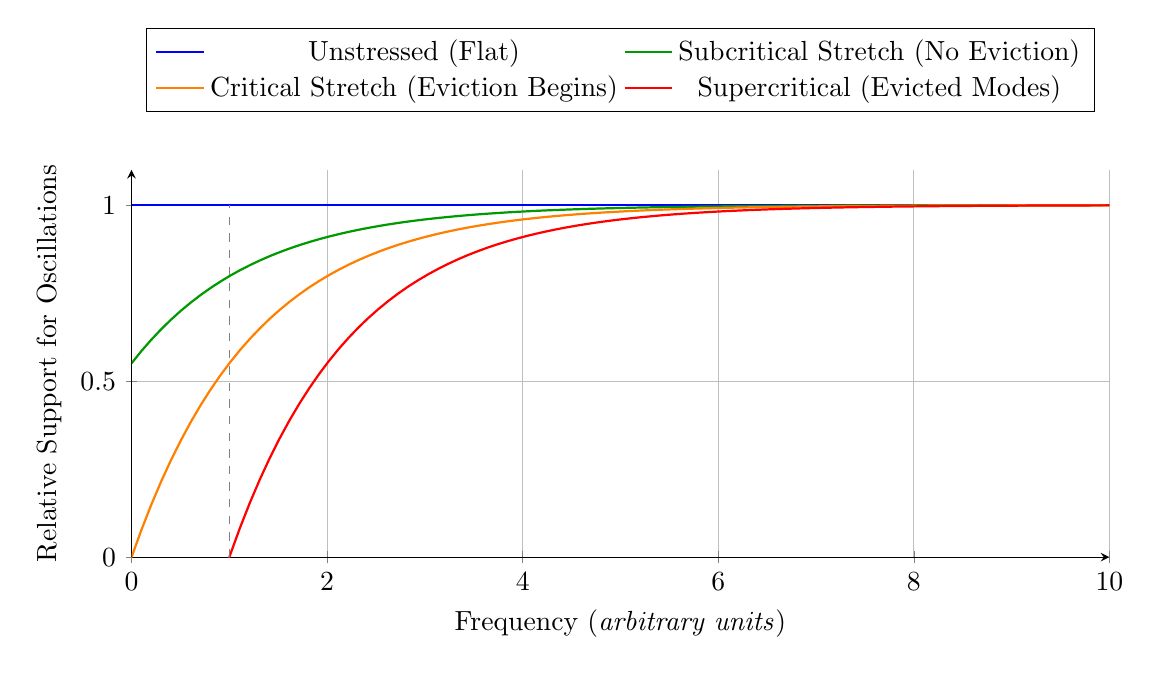
\begin{tikzpicture}
\begin{axis}[
    width=14cm,
    height=6.5cm,
    axis x line=bottom,
    axis y line=left,
    xmin=0, xmax=10,
    ymin=0, ymax=1.1,
    xtick={0,2,4,6,8,10},
    ytick={0,0.5,1.0},
    grid=both,
    xlabel={Frequency (\emph{arbitrary units})},
    ylabel={Relative Support for Oscillations},
    legend style={at={(0.5,1.15)},anchor=south,legend columns=2},
    clip=true
  ]

  % 1. Flat spacetime
  \addplot[domain=0:10, samples=100, thick, blue] {1};
  \addlegendentry{Unstressed (Flat)}

  % 2. Subcritical stretch - still supports all modes
  \addplot[domain=0:10, samples=100, thick, green!60!black] {1 - exp(-0.8*(x + 1))};
  \addlegendentry{Subcritical Stretch (No Eviction)}

  % 3. Critical stretch - touches origin
  \addplot[domain=0:10, samples=100, thick, orange] {1 - exp(-0.8*(x))};
  \addlegendentry{Critical Stretch (Eviction Begins)}

  % 4. Fully stretched - strong filtering
  \addplot[domain=0:10, samples=100, thick, red] {1 - exp(-0.8*(x -1))};
  \addlegendentry{Supercritical (Evicted Modes)}

  % Vertical line at critical threshold
  \draw[dashed, gray] (axis cs:1.0,0) -- (axis cs:1.0,1);

\end{axis}
\end{tikzpicture}
\caption{Effect of increasing spacetime tension on frequency support. Each curve represents a distinct tension regime, illustrating how lower-frequency modes are progressively suppressed as the stretch approaches and exceeds the critical limit.}
\label{fig:stretch-spectrum}\end{figure}

\newpage
Figure~\ref{fig:stretch-spectrum} illustrates how the frequency support of spacetime evolves under increasing tension. Each curve corresponds to a distinct physical regime:
\begin{itemize}
\item \textbf{Blue --- Unstressed (Flat):} All frequency modes are equally supported. No stretch or curvature is present. This is idealized Minkowski space.

\item \textbf{Green --- Subcritical Stretch:} Geometry begins favoring higher-frequency modes. Lower frequencies are disfavored but still supported---no evictions yet.

\item \textbf{Orange --- Critical Stretch:} The curve touches the origin, indicating the first suppression of zero-frequency modes. This marks the onset of rest-mass mode eviction at this spacetime stretch---shell formation begins.

\item \textbf{Red --- Supercritical Stretch:} Lower-frequency modes are actively excluded. Only high-energy or massless excitations remain sustainable in the interior. The shell is now fully formed.  The energy cutoff is shown here as a dashed vertical line.
\end{itemize}

This dynamic naturally explains surface-area scaling and shell-like mass distributions: low-frequency matter accumulates near the outer shell, while the interior is emptied of rest-mass content.  This mechanism is also consistent with entropy scaling: since low-frequency modes are excluded, the number of accessible interior microstates scales with surface area rather than volume.


\cleardoublepage
\part{Implications and Extensions}

\section{Observational and Experimental Consequences}

If the discrete standing wave model is to be more than a mathematical curiosity, it must leave its fingerprints on reality. Remarkably, several features long considered puzzles in the standard picture---from the ubiquity of supermassive black holes to the apparent acceleration of cosmic expansion---appear here as natural expectations. The following sections outline observational consequences, not as definitive predictions but as invitations to test the model against the cosmos itself.

\subsection{Gravitational Wave Ringdowns and Echoes}

Mergers of compact objects provide the most direct window into the strong-gravity regime. In classical general relativity, black holes exhibit damped quasinormal mode (QNM) ringdowns that depend only on mass and spin. In contrast, a shell-based compact object could support:

\begin{itemize}
    \item \textbf{Modified QNM spectra}, with additional or shifted resonant frequencies.
    \item \textbf{Echoes} in the post-merger signal, arising from reflections at the hard inner boundary.
    \item \textbf{Extended ringdown tails}, modulated by the mechanical response of the shell.
\end{itemize}

Future detectors such as LISA may have sufficient sensitivity to identify such deviations, providing a sharp observational discriminator.

\subsection{Accretion and Electromagnetic Signatures}

Infalling matter interacts differently with a hard surface than with an event horizon. This may produce:

\begin{itemize}
    \item \textbf{Hard surface emissions}, where accreted material deposits energy onto the shell, generating thermal radiation or high-energy bursts.
    \item \textbf{Quasi-steady boundary layers}, potentially visible in X-ray spectra.
    \item \textbf{Time-variable hotspots}, tied to surface inhomogeneities or oscillations.
\end{itemize}

Comparisons of accretion efficiencies between candidate black holes and neutron stars may already hint at such possibilities. High-resolution imaging (e.g., from the Event Horizon Telescope) could provide direct constraints.

\subsection{Surface Oscillations and QNMs}

The shell surface itself may host interface waves or pressure oscillations absent in classical horizons. These could couple to both gravitational and electromagnetic channels, producing:

\begin{itemize}
    \item Distinctive QNM ringdown structures.
    \item Modulations in post-merger signals.
\end{itemize}

Where GR predicts silence beyond the standard QNM spectrum, a Black Surface acts as a resonant drumhead, inviting search for oscillatory fingerprints that classical horizons cannot provide.

\subsection{Information and Interior Access}

The absence of a singularity reframes the black hole information paradox. A Black Surface replaces the featureless horizon with a physical interface, introducing new possibilities for information retention and recovery:

\begin{itemize}
    \item The shell may act as a reflective boundary preserving quantum correlations.
    \item The interior could be Minkowski vacuum, or some exotic phase, allowing partial recovery of information.
    \item Unlike ``firewall'' proposals, the surface offers a geometric rather than ad hoc resolution.
\end{itemize}

This connects naturally to the ``soft hair'' proposal of Hawking, Perry, and Strominger~\cite{hawking2016soft,hawking2018soft}, where information about infalling matter is stored in subtle supertranslation and superrotation charges on the horizon. While mathematically elegant, the soft-hair framework leaves open the question of what physical substrate actually carries these degrees of freedom, since the event horizon itself has no material form. In contrast, the Black Surface picture supplies a concrete boundary---a shell at the limit of spacetime stretch---on which such modes could reside. In this sense, the two ideas are complementary: soft hair provides the symmetry structure, while the Black Surface provides the physical seat.

Together, these perspectives suggest that black holes (or their replacements) may not be information sinks but resonant, memory-bearing systems, where horizon-scale structures encode and possibly re-emit quantum information. What appears paradoxical in standard GR becomes, in this framework, the expected behavior of a physical boundary.

\subsection{Primordial Black Holes and Seeds}

One striking observational fact is that nearly every galaxy hosts a supermassive black hole (SMBH) at its center. Their ubiquity is puzzling in standard cosmology: why should such rare, extreme objects become the rule rather than the exception?

In the standing-wave spacetime framework, the puzzle takes on a natural resolution. Because the effective coupling 
\[
\kappa(V) = \frac{8\pi G}{c(V)^4}
\]
was vastly larger in the early universe, gravity was overwhelmingly stronger at small cosmic volume. Collapse thresholds were lower, making the formation of primordial black holes (PBHs) far more common than in constant-$c$ cosmology. Even modest density fluctuations could seed collapse.

As the universe expanded and $c(V)$ grew, the effective strength of gravity diminished. Black holes did not need to accrete to appear larger relative to their environment: the decreasing coupling itself ``ballooned'' their effective horizon scale. In this sense, supermassive black holes could emerge not only through feeding but through the natural weakening of gravity over time.

Thus, the near-universal presence of SMBHs in galactic centers may not be an accident but a built-in feature of cosmic evolution. Billions of galaxies, each anchored by an early-formed compact seed, are a fossil record of gravity’s shifting strength. What seems exceptional in the standard picture becomes expected in a universe where gravity itself dilutes with volume.

\subsection{Open Problems and Research Directions}

The above should not be read as firm predictions, but as fertile research directions. A non-exhaustive list includes:

\begin{enumerate}
    \item \textbf{QNM and echo analyses}, searching gravitational wave data (LIGO/Virgo, and especially LISA) for non-Kerr structures.
    \item \textbf{High-precision accretion modeling}, incorporating hard boundaries into X-ray and EHT studies.
    \item \textbf{Numerical modeling of matter shells}, within both classical and modified GR frameworks.
    \item \textbf{Exploration of shell mechanics and energy conditions}, particularly in dynamical collapse scenarios.
\end{enumerate}

Together, these constitute perhaps the most testable implications of the discrete standing wave model.

\section{Open Questions and Theoretical Tensions}

If Part III set out the architecture of a discrete standing wave spacetime, and the previous section traced its observational fingerprints, the present section steps back. It asks not what the model \emph{predicts}, but what it \emph{requires}. The questions below are not failures but frontiers: invitations to mathematical refinement, physical insight, and perhaps even experimental discovery.

\subsection{Is a Reformulation of Quantum Mechanics Required?}

Quantum theory presumes a continuous background for wavefunction evolution, with time treated as a smooth parameter. If time instead emerges from an oscillatory, discrete substrate, can the Schrödinger equation still apply? Or must a new operator formalism be constructed, one adapted to a fundamentally discrete temporal flow?

\subsection{How Does Gravity Arise from Discrete Geometry?}

Here, gravity emerges not as a force but as a pressure gradient driven by temporal differentials. Yet a first-principles derivation remains absent. Is there a discrete analog to curvature, or to the stress-energy tensor, from which field equations can be derived? This is essential for a full reconciliation with general relativity.

\subsection{What Role does Higgs Field play?}

If inertial mass results from impedance against spacetime oscillation, the Higgs mechanism may itself be secondary. Is the Higgs field simply another standing wave mode? If so, this could recast spontaneous symmetry breaking not as a brute fact, but as a resonance phenomenon within the fabric of spacetime.

\subsection{Can Vacuum Energy Be Regularized?}

The vacuum energy catastrophe reflects a failure of continuum theory. In a discrete standing wave model, both a minimum frequency and a maximum warp depth exist. These natural cutoffs may eliminate infinitesimal mode contributions, suggesting a route to resolving the paradox. What appears catastrophic in the continuum may be regulated naturally by discreteness.

\subsection{Is Redshift Partially Misattributed?}

If $c = c(V)$, then cosmic redshift may not arise solely from metric expansion. Some fraction could reflect historical variation in $c$, lessening or removing the need for dark energy. The possible convexity of supernova Hubble plots may hint at precisely this effect. Thus, the very evidence once taken as proof of a cosmological constant may instead be the fossil record of a changing $c$.

\subsection{How Does Information Escape a Black Surface?}

Unlike an event horizon, a Black Surface is a finite shell. If the interior is not a true void, tunneling or resonant leakage may allow information escape, preserving unitarity without paradox. What appears impossible in GR---information recovery---becomes a natural consequence of a surface with physical structure.

\subsection{Does Discreteness Imply a Preferred Scale?}

A fundamental oscillation frequency might define a cosmological frame, apparently at odds with relativity. Yet local Lorentz invariance may survive as an emergent property of the wave structure, just as fluid dynamics inherits Galilean symmetry despite molecular discreteness.

\subsection{Is There a Boundary to the Wave Domain?}

A standing wave requires boundary conditions. What sets these in an expanding universe? Possibilities include holographic boundaries, topological closure, or embedding in a higher-dimensional domain. The observable universe may itself be only a subharmonic of a larger wave domain.

\subsection{Is This Model Testable?}

Ultimately, a theory stands or falls by experiment. Observable signatures may include:

\begin{itemize}
    \item Gravitational lensing near Black Surfaces deviating from Kerr predictions.
    \item Primordial light or gravitational waves exhibiting coherence limits inconsistent with a continuous metric.
    \item QNM ringdowns with echo structures absent from general relativity.
\end{itemize}

\vspace{2em}

\begin{center}
\textbf{Discreteness is either invisible---or it is everything.}
\end{center}


---


\newpage
\bibliographystyle{unsrtnat}  % Updated to ensure citations are in appearance order
\bibliography{references}

\end{document}

